\documentclass[11pt]{article}

\usepackage[margin=1in]{geometry}
\usepackage{amsfonts,amsmath}
\usepackage{booktabs}
\usepackage{multirow}
\usepackage{graphicx}
\usepackage{xcolor}
\usepackage[colorlinks,citecolor=blue,urlcolor=blue,linkcolor=blue]{hyperref}
\usepackage[numbers,sort&compress]{natbib}
\usepackage[affil-it]{authblk}
\usepackage{lineno}

\renewcommand{\arraystretch}{1.3}
\emergencystretch=1.5em

\newcommand{\Gr}{\mathrm{Gr}}
\newcommand{\R}{\mathbb{R}}

\title{Construct Validity Failure in Single-Cell Embedding Evaluation:\\
Null Saturation Bounds and Source Classifier Confidence}

\author{Elliot Tower}
\affil{Independent researcher \\ \texttt{elliot@elliottower.ai}}
\date{}

\begin{document}
\linenumbers
\maketitle

\begin{abstract}

\textbf{Background:}
Single-cell foundation model benchmarks consistently report that PCA
on raw counts matches or exceeds large pretrained embeddings across
most evaluation axes. Whether this reflects a genuine limitation of
current models or a construct validity failure in the evaluation
metrics remains unresolved. Existing metrics conflate two logically
independent tasks---ranking models against each other and certifying
that a model captures biological signal---and a metric can succeed at
one while failing at the other.

\textbf{Results:}
We evaluated twelve metrics against cross-technology cell-type
transfer F1 (classifier trained on 10x Chromium 3$'$ v3 embeddings,
applied to Smart-seq2) across 23 human tissues and 92 embedding
conditions in CELLxGENE Census. Centered kernel alignment (CKA) on
cell-type centroids retains ranking power (partial $\rho = 0.53$,
controlling for dimensionality) yet exhibits what we term \emph{null saturation}:
its analytic expectation under a Gaussian null,
$\mathbb{E}[\mathrm{CKA}] \approx 1 - 1.06\,(k{-}1)/(d{+}k)$,
exceeds every trained-model score at foundation-model dimensionality.
At $d = 50$, 86\% of conditions across four datasets clear the null;
at $d \geq 512$, none do. CKA's ranking ability replicates on two
independent datasets (pancreas, Tabula Sapiens) but not a third
(PBMC) where cell-type classification is uniformly easy. Five
relational consistency score variants and pairwise discrimination
accuracy avoid null saturation yet predict transfer only marginally
($\rho \leq 0.25$). These failures share a mechanism: relational
metrics measure geometric similarity between cell-type relationship
matrices, which does not reflect cluster separability. Source
classifier confidence (SCC)---the mean maximum predicted probability
of a source-trained cell-type classifier applied to target
cells---directly measures whether learned decision boundaries
transfer, achieving Spearman $\rho = 0.67$ ($p < 10^{-13}$,
BH-corrected across twelve metrics, four embedding models). A
pre-registered cross-classifier stress test confirms this result
across four classifier families, ruling out shared-machinery
confounding. SCC also predicts marker gene recovery---a
non-classification ground truth scored in gene space via Leiden
clustering---with Spearman $\rho = 0.32$ (block-bootstrap 95\% CI
$[0.15, 0.44]$), providing convergent validity from a structurally
distinct evaluation pathway.

\textbf{Conclusions:}
Relational embedding metrics quantify geometric fidelity, which does
not capture the cluster separability that determines downstream
cell-type classification performance. SCC provides a practical
alternative for predicting cross-assay transfer, robust across
classifier families and validated against a non-classification ground
truth. Benchmark rankings derived from relational
metrics alone do not reliably reflect differences in biological signal
capture; published comparisons between foundation models and simple
baselines warrant re-evaluation with transfer-aware metrics.

\end{abstract}

\noindent\textbf{Keywords:} single-cell foundation models, embedding evaluation, construct validity, centered kernel alignment, source classifier confidence, transfer prediction

\section{Introduction}
\label{sec:intro}

Single-cell foundation model benchmarks consistently find that PCA on
raw counts matches or exceeds large pretrained models across most
evaluation axes \citep{wu2025scfm, vcbench2026, unifiedscfm2026,
cellxgeneintegration2026, chen2026harmonised, liu2026zeroshot}. \citet{wu2025scfm} raised the possibility
that the metrics themselves might be at fault. The question is whether
high metric scores reflect biological signal learned by the model, or
geometric properties that arise in any high-dimensional embedding. This is
a question of \emph{construct validity}---whether a measure tracks the
property it is intended to track rather than something correlated with
it \citep{cronbach1955construct}---asked of a benchmark suite rather than
of a psychological test.

Embedding metrics serve two roles that the field treats as one. The
first is \emph{ranking}: given two trained models, which produces a
better embedding? The second is \emph{certification}: does a given
model capture biological signal at all? These are logically independent.
A metric can rank trained models correctly while scoring all of them
below unstructured random noise, or it can separate trained from random
while failing to rank among trained models. Treating one as evidence for
the other conflates two distinct claims about metric quality. Separating
what a measure shares with its intended construct from what it shares with
the procedure used to compute it is the problem \citet{campbell1959convergent}
posed for psychological measurement; the metrics below are audited in those
terms.

We evaluate twelve metrics spanning three families---scIB
bio-conservation \citep{luecken2022scib}, cell-type centroid alignment,
and five geometric modules---on 104 embedding conditions across 25
tissues. Ground truth is cross-technology cell-type transfer F1 from
10x Chromium 3$'$ v3 to Smart-seq2.

Seven findings emerge. First, most metrics rank well: Procrustes
similarity on cell-type centroids achieves partial $\rho = +0.66$ with
downstream transfer, and nine of twelve metrics reach significance after
controlling for dimensionality. Second, CKA exhibits null saturation---the
analytic null is a closed-form function of $k$ and $d$:
$\mathbb{E}[\mathrm{CKA}] \approx 1 - 1.06\,(k{-}1)/(d{+}k)$. This
formula places the boundary between regimes where CKA can and cannot
certify: at $d = 50$, 86\% of conditions across four datasets clear the
null; at $d \geq 512$, none do. PCA-reduction and random projection
controls confirm that dimensionality reduction accounts for the majority
of the effect, with a measurable denoising component (PCA clears 59\%
vs.\ random projections 46--48\%). Third, relational consistency scores
(RCS), which operate on $k \times k$ cell-type relationship matrices,
are dimensionality-stable and discriminate embedding quality, but
achieve only marginal transfer prediction ($\rho = 0.25$). Fourth,
source classifier confidence (SCC)---the mean maximum predicted
probability of a source-trained classifier applied to target
data---achieves $\rho = 0.67$ with transfer F1 ($p < 10^{-13}$,
BH-corrected across twelve metrics) across four embedding models and
92 conditions; a cross-classifier stress test confirms this is an
embedding-space property, not a classifier artifact. SCC also predicts
marker gene recovery ($\rho = 0.32$, block-bootstrap CI
$[0.15, 0.44]$), a non-classification ground truth, providing
convergent validity. Fifth, two attempted
repairs fail in diagnosable ways: a spectral-gap statistic inverts
(null baselines more concentrated than trained models),
and $z$-score normalization degrades ranking by removing real
$k$-dependent signal. Sixth, multi-seed noise calibration (10 seeds, 22
tissues) shows that apparent non-monotonicity in Leiden-dependent
bio-conservation metrics is clustering jitter: ARI drops from 70\% to
6.7\% non-monotonic after permutation calibration (10.5$\times$
inflation). Seventh, a cross-tissue replication experiment localizes the
ranking failure: scIB metrics achieve 22\% pairwise inversions on
cross-tissue transfer ($\rho = +0.63$, $p = 0.0014$), compared with
30--48\% in the cross-assay setting where protocol artifacts confound.

These findings yield both a usability criterion and a constructive
alternative. Given $k$ shared cell types and dimension $d$, compute the
analytic null; if the expected effect size does not exceed it, CKA is
uninformative as a certification tool. Every current single-cell
foundation model operates in the regime where this criterion is
violated. For predicting transfer quality directly, SCC provides the
strongest single statistic ($\rho = 0.67$ across four embedding
models, with convergent validity from a non-classification ground
truth).


\section{Results}

\subsection{Evaluation panel}
\label{sec:panel}

We constructed a cross-technology transfer panel from CellxGene Census
(v2023-12-15). Source embeddings are computed on 10x Chromium 3$'$ v3
cells; target labels come from Smart-seq2 (EFO:0008931) cells in the
same tissue with zero donor overlap. Tissues were auto-discovered by
requiring $\geq 200$ cells per assay and $\geq 8$ shared cell types,
yielding 25 tissues. Eight embedding models
span three architectural families, at their Census-hosted dimensionalities:
Geneformer \citep{theodoris2023geneformer} ($d = 512$), Geneformer-v2 104M and 316M, scGPT \citep{cui2024scgpt}
($d = 512$), scVI \citep{lopez2018scvi} ($d = 50$), bag-of-genes
PCA-512 ($d = 512$; following \citealp{cole2026morpheus}), random
Gaussian projection ($d = 512$), and an untrained two-layer MLP encoder
($d = 512$). Six contender models (excluding the two null baselines)
produce 104 contender conditions. Ground truth is macro-averaged
logistic-regression F1 on shared cell types, trained on source
embeddings and evaluated on target.


\subsection{Metric prediction of cross-technology transfer}
\label{sec:prediction}

Twelve metrics were evaluated on all 104 contender conditions. Partial
Spearman rank correlations control for embedding dimensionality via rank
residuals from OLS; tissue-stratified permutation tests (10,000
iterations) provide $p$-values robust to within-tissue dependence.

Nine of twelve metrics significantly predict cross-technology transfer
(Table~\ref{tab:metrics}). Procrustes similarity on cell-type centroids
achieves the strongest correlation (partial $\rho = +0.66$,
$p < 10^{-13}$), followed by target-domain silhouette ($\rho = +0.65$)
and silhouette on cell-type labels ($\rho = +0.60$). Cell-type CKA
achieves $\rho = +0.53$ ($p < 10^{-8}$). Among scIB metrics, graph
connectivity ($\rho = +0.58$), NMI ($\rho = +0.55$), and kNN purity
($\rho = +0.52$) predict transfer at comparable strength. ARI predicts
more weakly ($\rho = +0.37$). The three failures are
direction stability ($\rho = +0.02$, $p = 0.83$) and
participation ratio ($\rho = +0.45$, nominally significant but
confounded by dimensionality; Supplementary~\ref{app:modules}).

\medskip
\begin{table}[t]
\centering
\caption{Partial Spearman correlation of twelve embedding metrics with
cross-technology transfer F1 ($n = 104$ contender conditions, 25
tissues). Controlling for embedding dimensionality $d$; $p$-values from
tissue-stratified permutation (10,000 iterations). Metrics ranked by
$|\rho|$. Bold: $p < 0.001$.}
\label{tab:metrics}
\small
\begin{tabular}{@{}lccl@{}}
\toprule
Metric & Partial $\rho$ & Perm.\ $p$ & Family \\
\midrule
Procrustes similarity   & $+0.652$ & $\mathbf{< 10^{-4}}$ & centroid \\
Silhouette (target)     & $+0.647$ & $\mathbf{< 10^{-4}}$ & scIB bio \\
Silhouette (label)      & $+0.599$ & $\mathbf{< 10^{-4}}$ & scIB bio \\
Graph connectivity      & $+0.579$ & $\mathbf{< 10^{-4}}$ & scIB bio \\
NMI (Leiden)            & $+0.553$ & $\mathbf{< 10^{-4}}$ & scIB bio \\
Cell-type CKA           & $+0.530$ & $\mathbf{< 10^{-4}}$ & centroid \\
kNN purity              & $+0.515$ & $\mathbf{< 10^{-4}}$ & scIB bio \\
cLISI                   & $+0.493$ & $\mathbf{< 10^{-4}}$ & scIB bio \\
Participation ratio     & $+0.450$ & $\mathbf{< 10^{-4}}$ & geometric \\
Isolated label ASW      & $+0.425$ & $\mathbf{< 10^{-4}}$ & scIB bio \\
ARI (Leiden)            & $+0.368$ & $\mathbf{< 10^{-4}}$ & scIB bio \\
Direction stability     & $+0.022$ & $0.83$               & geometric \\
\bottomrule
\end{tabular}
\end{table}

Controlling for both dimensionality and the number of shared cell types
attenuates correlations by $\leq 3\%$ (CKA: $\rho = 0.52$; Procrustes:
$\rho = 0.64$), confirming that the predictions are driven by embedding
quality rather than panel structure.


\subsection{CKA null saturation is a function of dimensionality}
\label{sec:nullfloor}

Predictive validity does not imply discriminative validity. We
constructed a null baseline by generating pairs of random Gaussian
centroid matrices ($k \times d$, entries $\sim \mathcal{N}(0,1)$) and
computing CKA and Procrustes similarity. The expected CKA under this
null admits a closed-form expression via Wishart moments
(Methods~\ref{sec:closedform}):
\begin{equation}
\label{eq:cka_null}
\mathbb{E}[\mathrm{CKA}(X, Y)] \approx 1 - 1.06 \cdot \frac{k-1}{d+k}
\end{equation}
This formula matches simulation within 0.02\% across $k = 8$--$44$
(Table~\ref{tab:nullfloor}). The formula depends only on $k$ and $d$,
so the analytic null is determined by the embedding dimension and the
number of cell types, independent of the model, tissue, or biology.

The formula reveals that null saturation is not constant: it weakens
as $d$ decreases. At $d = 512$, $k = 16$, the null is 0.970; at
$d = 50$, $k = 16$, it drops to 0.772. To push the null below the
observed CKA mean of 0.74 requires $k > 168$ shared cell types at
$d = 512$, $k > 66$ at $d = 200$, and only $k > 18$ at $d = 50$
(Table~\ref{tab:crossover}). No single-cell dataset has 168 shared cell
types across technology pairs, so CKA at $d = 512$ is confounded by
construction.

\medskip
\begin{table}[t]
\centering
\caption{The analytic null as a function of $d$ and $k$.
$\mathbb{E}[\mathrm{CKA}] \approx 1 - 1.06\,(k{-}1)/(d{+}k)$,
verified by simulation (1,000 draws per cell). Null saturation tightens
monotonically with $d/k$; at foundation-model dimensionalities
($d \geq 512$), the analytic null exceeds all observed embedding CKA scores.}
\label{tab:nullfloor}
\small
\begin{tabular}{@{}rcccc@{}}
\toprule
& \multicolumn{4}{c}{Analytic CKA null at dimension $d$} \\
\cmidrule(lr){2-5}
$k$ & $d = 50$ & $d = 200$ & $d = 512$ & $d = 1280$ \\
\midrule
8  & 0.872 & 0.964 & 0.986 & 0.994 \\
14 & 0.785 & 0.936 & 0.974 & 0.989 \\
22 & 0.691 & 0.900 & 0.958 & 0.983 \\
44 & 0.515 & 0.813 & 0.921 & 0.965 \\
\bottomrule
\end{tabular}
\end{table}

\medskip
\begin{table}[t]
\centering
\caption{Crossover: number of shared cell types $k$ needed for the
analytic null to drop below the observed CKA mean of 0.74, as a function
of embedding dimension $d$.}
\label{tab:crossover}
\small
\begin{tabular}{@{}rrl@{}}
\toprule
$d$ & $k$ needed & Feasibility \\
\midrule
50   & $> 18$  & Routine \\
200  & $> 66$  & Rare but achievable \\
512  & $> 168$ & Beyond any existing dataset \\
1280 & $> 417$ & Infeasible \\
\bottomrule
\end{tabular}
\end{table}


\subsection{Discriminability across dimensionality regimes}
\label{sec:deffect}

The analytic null generates a testable prediction: conditions at low $d$
should clear the analytic null, while conditions at high $d$ should not. We
tested this across four datasets spanning $d = 50$ to $d = 1{,}152$
(Table~\ref{tab:deffect}). At $d = 50$, 218 of 253 conditions (86\%)
exceed their $(k, d)$-matched null. At $d = 200$, 76 of 456 (17\%).
At $d \geq 512$, zero of 129. The gradient is monotone across four
levels of $d$ and holds within each dataset independently.

\medskip
\begin{table}[t]
\centering
\caption{Fraction of conditions exceeding the analytic CKA null, by
embedding dimension. Four datasets: Census (25 tissues, 8 models),
pancreas (56 pairs), Tabula Sapiens (16 pairs), PBMC (42 pairs).}
\label{tab:deffect}
\small
\begin{tabular}{@{}rrrrl@{}}
\toprule
$d$ & Above null & Total & \% above & Source \\
\midrule
50   & 218 & 253 & 86.2 & Census (scVI) + external PCA \\
200  &  76 & 456 & 16.7 & External PCA/random \\
512  &   0 & 125 &  0.0 & Census (all $d{=}512$ models) \\
$\geq 768$ & 0 & 4 & 0.0 & Census (Geneformer-v2) \\
\bottomrule
\end{tabular}
\end{table}

This gradient could reflect dimensionality or model family, since the
$d = 50$ conditions include scVI and PCA while the $d = 512$ conditions
include foundation models and PCA. A within-panel comparison breaks
this confound. scVI is a foundation model (variational autoencoder
trained on millions of cells) that outputs $d = 50$ embeddings; it
clears the null in 16 of 25 tissues. Bag-of-genes PCA at $d = 512$---a
classical method, not a foundation model---fails in all 25
(Table~\ref{tab:confound}). Both model families fail at $d = 512$; the
foundation model succeeds at $d = 50$. Dimensionality is the causal
variable.

\medskip
\begin{table}[t]
\centering
\caption{Confound control: model family vs.\ dimensionality. Fraction of
25 tissues where CKA exceeds the analytic null. Rows: model family.
Columns: embedding dimension.}
\label{tab:confound}
\small
\begin{tabular}{@{}lcc@{}}
\toprule
& $d = 50$ & $d = 512$ \\
\midrule
Foundation model & scVI: 16/25 (64\%) & Geneformer: 0/25 (0\%) \\
PCA / random     & (external: 86\%)   & BoG-PCA: 0/25 (0\%) \\
\bottomrule
\end{tabular}
\end{table}

A PCA-reduction control confirms this. Geneformer ($d = 512$) and
scGPT ($d = 512$) cell-level embeddings were PCA-reduced to $d = 50$
and $d = 200$ (joint PCA on source and target cells), and CKA was
recomputed against the $(k, d_{\mathrm{reduced}})$ null. At native
$d = 512$, Geneformer clears the null in 0/22 tissues and scGPT in
0/22. After reduction to $d = 50$, Geneformer clears 18/22 (82\%) and
scGPT 8/22 (36\%). At $d = 200$, Geneformer clears only 2/22 and scGPT
0/22 (Table~\ref{tab:pca_reduction}). The same embeddings, from the
same model, cross the certification boundary when their dimensionality
crosses it. Model architecture is held constant; dimensionality is the
causal variable.

\medskip
\begin{table}[t]
\centering
\caption{PCA-reduction confound control. Fraction of 22 tissues where
CKA exceeds the $(k, d)$-matched analytic null, by model and
dimensionality. scVI ($d = 50$) shown for reference (no reduction
applied).}
\label{tab:pca_reduction}
\small
\begin{tabular}{@{}lccc@{}}
\toprule
Model & Native $d$ & $d = 50$ & $d = 200$ \\
\midrule
Geneformer      & 0/22 (0\%)  & 18/22 (82\%) & 2/22 (9\%) \\
scGPT           & 0/22 (0\%)  & 8/22 (36\%)  & 0/22 (0\%) \\
scVI (ref.)     & 15/22 (68\%) & ---         & --- \\
\bottomrule
\end{tabular}
\end{table}

Null-normalizing CKA by subtracting the analytic mean and dividing by
the null standard deviation weakens rather than improves predictive
validity ($z$-CKA: $\rho = +0.42$ vs.\ raw CKA $\rho = +0.46$;
partial $\rho|d$: $0.39$ vs.\ $0.44$). Within the $d = 50$ stratum,
the degradation is larger ($\rho = +0.17$ vs.\ $+0.45$): $z$-scoring
removes the $k$-dependent signal that CKA carries at low $d$, where the
metric has real discriminative power. The normalization is actively
harmful in the regime where CKA works and redundant in the regime where
it does not. The constructive fix is the usability criterion itself,
not a rescaled score.


\subsection{Random projection control: denoising versus dimensionality reduction}
\label{sec:randproj}

The PCA-reduction control shows that reducing $d = 512$ embeddings to
$d = 50$ recovers CKA discriminability. PCA both reduces dimensionality
and denoises (retaining variance-ordered components), so the recovery
could reflect either mechanism. A random projection control isolates
pure dimensionality reduction from denoising.

For each tissue, Geneformer and scGPT embeddings ($d = 512$) were
projected to $d_{\mathrm{out}} \in \{50, 200\}$ via three methods:
PCA (joint, reproducing the preceding control), Gaussian random
projection ($R \in \R^{d_{\mathrm{out}} \times 512}$,
$R_{ij} \sim \mathcal{N}(0, 1/d_{\mathrm{out}})$), and orthogonal
random projection (QR decomposition of a Gaussian matrix). Ten
independent seeds were drawn per condition; reported CKA values are
seed means.

\medskip
\begin{table}[t]
\centering
\caption{Fraction of 44 conditions (22 tissues $\times$ 2 models) where
CKA exceeds the $(k, d)$-matched analytic null, by projection method and
target dimension. None clears the 60\% threshold.
Gaussian and orthogonal projections are interchangeable (mean
$|\Delta\text{CKA}| = 0.015$ at $d = 50$).}
\label{tab:randproj}
\small
\begin{tabular}{@{}lcccc@{}}
\toprule
Method & $d$ & Above null & Rate & Mean CKA \\
\midrule
PCA              & 50  & 26/44 & 59.1\% & $0.786 \pm 0.142$ \\
Gaussian         & 50  & 21/44 & 47.7\% & $0.748 \pm 0.127$ \\
Orthogonal       & 50  & 20/44 & 45.5\% & $0.756 \pm 0.126$ \\
\midrule
PCA              & 200 &  2/44 &  4.5\% & $0.794 \pm 0.138$ \\
Gaussian         & 200 &  1/44 &  2.3\% & $0.782 \pm 0.134$ \\
Orthogonal       & 200 &  2/44 &  4.5\% & $0.786 \pm 0.136$ \\
\midrule
Native           & 512 &  0/44 &  0.0\% & $0.795 \pm 0.150$ \\
\bottomrule
\end{tabular}
\end{table}

No projection method clears the 60\% threshold
(Table~\ref{tab:randproj}). PCA achieves the highest recovery at
$d = 50$ (59.1\%), followed by Gaussian (47.7\%) and orthogonal
(45.5\%) random projections. The 12-percentage-point gap between PCA
and random projections quantifies PCA's denoising contribution:
variance-ordered component selection retains more cell-type structure
than random linear combinations at the same target dimension.

Gaussian and orthogonal projections produce nearly identical results
(mean $|\Delta\text{CKA}| = 0.015$ at $d = 50$, max $0.047$),
confirming that the effect is geometric---determined by the target
dimension. At $d = 200$, all three methods collapse to near-zero
clearance (2--5\%), confirming the analytic null's $d$-dependence even for
reduced embeddings.

Geneformer benefits substantially from $d$-reduction (73--82\% clearance
at $d = 50$ across methods). scGPT benefits less (18--36\%), consistent
with its lower transfer F1 leaving less cell-type structure to preserve
under projection.


\subsection{Relational consistency scores: dimensionality-stable but weakly predictive}
\label{sec:scgraph}

The preceding results establish that CKA cannot certify biological
signal at $d \geq 512$, and that dimensionality reduction only
partially recovers certification ability. An alternative metric immune
to $d$-dependent null saturation would bypass the problem entirely.
Relational consistency scores (RCS), following the approach of scGraph
\citep{wang2026scgraph}, evaluate relational structure between cell
types via $k \times k$ relationship matrices---centroid distance
correlations, $k$NN overlap, and weighted affinity---then correlate the
upper-triangular entries across assays. Because these metrics operate on
$k \times k$ matrices, they should be invariant to CKA null saturation
by construction.

All 22 tissues, three models (Geneformer $d = 512$, scGPT $d = 512$,
scVI $d = 128$), and three RCS variants were evaluated at native $d$
and at PCA-reduced $d = 50$ for the $d = 512$ models.

RCS is dimensionality-stable: the centroid distance correlation changes
by a median of only 0.017 between native $d = 512$ and PCA-reduced
$d = 50$ (IQR: 0.009--0.047), compared to CKA's analytic null shift
from 0.98 to 0.84 over the same range. RCS also discriminates embedding
quality: Geneformer produces higher RCS scores than scGPT in 17 of
22 tissues (77.3\%), matching the transfer-F1 ordering.

The dissociation is complete: 100\% of $d = 512$ conditions fall below
the CKA analytic null, yet 93\% produce RCS centroid distance
correlations $\geq 0.20$.

RCS's limitation is transfer prediction. The pooled Spearman correlation
between RCS and transfer F1 is marginal ($\rho = 0.25$, $p = 0.054$),
driven by between-model variance---Geneformer has both higher F1 and
higher RCS than scGPT. RCS tracks which model produces better relational
structure across assays; tissue-level variation within a model falls
outside its resolution. The failure is structural: Spearman correlation
on centroid distances is invariant to monotonic scaling, so an embedding
space where clusters overlap (low F1) scores identically to one where
clusters are well-separated (high F1), as long as relative distances are
preserved. This motivates a search for metrics that capture cluster
separability directly.


\subsection{Transfer-aware metrics recover prediction}
\label{sec:scc}

RCS's marginal F1 correlation ($\rho = 0.25$) motivates a search for
metrics that capture what relational structure misses: cluster
separability and conditional alignment.

Source classifier confidence (SCC) trains a cell-type classifier on
source embeddings, applies it to target cells, and reports the mean
maximum predicted probability. Four classifier families were tested
(logistic regression, kNN, random forest, linear SVM); F1 ground truth
always uses logistic regression. Maximum mean discrepancy (MMD) measures kernel-based
distributional divergence between source and target (Gaussian kernel,
median-heuristic bandwidth, PCA-50 reduced). Class-conditional alignment
(CCAL) averages, across shared cell types, $1 - \|c_s - c_t\| /
(\text{radius}_s + \epsilon)$ where $\text{radius}_s$ is the mean L2
distance of source cells to their centroid. Proxy A-distance (PAD)
trains a domain classifier to distinguish source from target cells.

\medskip
\begin{table}[t]
\centering
\caption{Transfer-aware metric comparison (23 tissues $\times$ 4
models, 92 conditions). Spearman $\rho$ with transfer F1, pairwise
model discrimination accuracy (binomial test), and within-tissue
Kendall $\tau$ sign test. All $p$-values BH-corrected across twelve
metrics. SCC variants use four classifier families; F1 ground truth
always uses logistic regression.}
\label{tab:scc}
\small
\begin{tabular}{@{}lcccccc@{}}
\toprule
Metric & Spearman $\rho$ & 95\% CI & $p_{\text{BH}}$ & Pairwise & $\tau$ (+/N) & $p_{\text{BH}}$ \\
\midrule
SCC (LR)         & $+0.673$ & $[+.54,\;+.78]$ & $<0.001$ & 77.5\% & 18/23 & $0.009$ \\
SCC (kNN)        & $+0.558$ & $[+.40,\;+.69]$ & $<0.001$ & 70.3\% & 16/23 & $0.062$ \\
SCC (RF)         & $+0.569$ & $[+.40,\;+.71]$ & $<0.001$ & 71.7\% & 18/23 & $0.009$ \\
SCC (SVM)        & $+0.548$ & $[+.37,\;+.70]$ & $<0.001$ & 68.1\% & 18/23 & $0.009$ \\
\midrule
MMD              & $+0.525$ & $[+.36,\;+.66]$ & $<0.001$ & 79.0\% & 20/23 & $0.001$ \\
CCAL             & $+0.472$ & $[+.30,\;+.62]$ & $<0.001$ & 75.4\% & 20/23 & $0.001$ \\
\midrule
RCS (baseline)   & $+0.218$ & $[+.02,\;+.40]$ & $0.050$  & 71.0\% & 16/23 & $0.062$ \\
RCS (PCA-10)     & $+0.284$ & $[+.07,\;+.48]$ & $0.009$  & 63.0\% & 14/23 & $0.221$ \\
RCS (trimmed)    & $+0.212$ & $[+.02,\;+.40]$ & $0.051$  & 71.7\% & 19/23 & $0.005$ \\
RCS (normalized) & $+0.179$ & $[-.03,\;+.38]$ & $0.096$  & 72.5\% & 18/23 & $0.009$ \\
RCS (combined)   & $+0.315$ & $[+.10,\;+.51]$ & $0.004$  & 63.0\% & 14/23 & $0.221$ \\
\midrule
PAD              & $+0.003$ & $[-.20,\;+.20]$ & $0.975$  & 46.5\% &  8/23 & $0.953$ \\
\bottomrule
\end{tabular}
\end{table}

SCC with logistic regression achieves the strongest pooled correlation
with F1 ($\rho = +0.67$, $p < 10^{-13}$, BH-corrected across twelve
metrics; Table~\ref{tab:scc}). Replacing the SCC classifier with
kNN ($\rho = +0.56$), random forest ($\rho = +0.57$), or linear SVM
($\rho = +0.55$) preserves the relationship, ruling out a shared-classifier
artifact: all four SCC variants pass BH correction.
MMD ($\rho = +0.53$) and CCAL ($\rho = +0.47$) produce concordant
results, providing convergent evidence from distributional-divergence
and centroid-alignment perspectives.

PAD---the metric most directly grounded in domain-adaptation
theory---fails entirely ($\rho = +0.003$, non-significant). PAD
measures marginal distributional alignment; two embedding spaces can have
identical marginal distributions yet completely different class-conditional
structure. SCC succeeds because classifier confidence integrates both
separability and conditional alignment into a single statistic: low
confidence arises precisely when target cells fall in ambiguous regions
of the learned decision space.

Ablations isolating the four differences between RCS and official scGraph
(dimensionality, centroid method, normalization, reference frame) show
that no single design choice explains the gap; all RCS variants
produce $\rho \in [0.18, 0.32]$, confirming that the RCS failure is
structural rather than a correctable implementation detail.


\subsection{Convergent validity: marker gene recovery}
\label{sec:mgr}

SCC's correlation with F1 could reflect shared classification
machinery rather than an embedding-space property that generalizes
beyond classifier transfer. To test this, we evaluated whether SCC
predicts marker gene recovery (MGR), a ground truth computed entirely
in gene space. MGR and transfer F1 share a construct and differ in
method, making this the monotrait-heteromethod comparison of
\citet{campbell1959convergent}: agreement across procedures with as
little shared machinery as possible is evidence that a measure tracks
the construct rather than a feature of one procedure.

MGR scores each embedding by whether Leiden clusters on target cells
recover the same differentially expressed genes found in the source
domain. Target cells are clustered by Leiden community detection on
the embedding's kNN graph; top-50 Wilcoxon rank-sum markers are
computed per cluster on raw counts and compared to reference markers
from source cell types via Jaccard overlap
(Methods~\ref{sec:mgrmethod}). The evaluation pathway shares no
classification machinery with SCC: Leiden community detection replaces
the trained classifier, Wilcoxon rank-sum on raw counts replaces
predicted probabilities, and Jaccard overlap of marker gene sets
replaces label agreement.

F1 and MGR are correlated but distinct ($\rho = 0.527$,
$p < 10^{-7}$), within the convergent-validity window
($\rho \in [0.25, 0.80]$): high enough to measure a related property,
low enough to constitute independent evidence.

SCC with logistic regression achieves $\rho = +0.318$ with MGR
(block-bootstrap 95\% CI $[0.150, 0.441]$;
Table~\ref{tab:mgr}). All four SCC variants reach BH significance,
occupying the top four positions by $|\rho|$ with MGR. SCC (kNN)
achieves the highest correlation ($\rho = +0.503$) but shares
neighborhood-graph machinery with Leiden clustering; the convergent
validity claim rests on SCC with logistic regression, whose linear
decision boundaries are structurally independent of Leiden's community
detection. MMD is the only non-SCC metric to survive BH correction
($\rho = +0.278$, $p_{\text{BH}} = 0.018$). CCAL, which correlates
moderately with F1 ($\rho = 0.47$), does not correlate with MGR
($\rho = 0.03$, $p = 0.80$), indicating that centroid alignment
captures classifier-relevant structure but not gene-level signal
recovery.

A ceiling control using true target labels instead of Leiden clusters
yields mean MGR of 0.20, representing the maximum achievable marker
recovery given cross-assay expression shift alone. The moderate
SCC--MGR effect sizes ($\rho = 0.32$--$0.50$) are consistent with
this ceiling: most marker divergence reflects technology-driven
expression shift rather than embedding quality. Leave-one-out
recomputation (dropping each tissue in turn) confirms robustness: the
bootstrap CI lower bound remains above zero for all 23 single-tissue
removals, with maximum $|\Delta\rho| = 0.059$.

\medskip
\begin{table}[t]
\centering
\caption{Correlation of twelve metrics with marker gene recovery
(MGR) across 92 conditions (23 tissues $\times$ 4 models). Spearman
$\rho$ with block-bootstrap 95\% CI (resampling tissues, 10{,}000
draws). $p$-values BH-corrected across twelve metrics. Bold:
$p_{\text{BH}} < 0.05$. SCC (kNN) shares neighborhood-graph
machinery with the Leiden clustering used to compute MGR.}
\label{tab:mgr}
\small
\begin{tabular}{@{}lccc@{}}
\toprule
Metric & Spearman $\rho$ & 95\% CI & $p_{\text{BH}}$ \\
\midrule
SCC (kNN)$^\dagger$  & $+0.503$ & $[+.20,\;+.71]$ & $\mathbf{<0.001}$ \\
SCC (SVM)            & $+0.433$ & $[+.11,\;+.64]$ & $\mathbf{<0.001}$ \\
SCC (RF)             & $+0.329$ & $[+.13,\;+.47]$ & $\mathbf{0.005}$ \\
SCC (LR)             & $+0.318$ & $[+.15,\;+.44]$ & $\mathbf{0.006}$ \\
\midrule
MMD                  & $+0.278$ & $[+.04,\;+.48]$ & $\mathbf{0.018}$ \\
RCS (combined)       & $+0.244$ & $[-.01,\;+.49]$ & $\mathbf{0.038}$ \\
\midrule
RCS (PCA-10)         & $+0.213$ & $[-.06,\;+.48]$ & $0.070$ \\
RCS (baseline)       & $+0.198$ & $[-.12,\;+.50]$ & $0.089$ \\
RCS (trimmed)        & $+0.190$ & $[-.14,\;+.50]$ & $0.094$ \\
RCS (normalized)     & $+0.142$ & $[-.20,\;+.46]$ & $0.212$ \\
CCAL                 & $+0.027$ & $[-.16,\;+.26]$ & $0.799$ \\
PAD                  & $-0.065$ & $[-.23,\;+.08]$ & $0.584$ \\
\bottomrule
\multicolumn{4}{@{}l@{}}{$^\dagger$Shares kNN-graph machinery with Leiden; not used for convergent validity argument.}
\end{tabular}
\end{table}


\subsection{Null saturation is structural; Leiden metrics show clustering jitter}
\label{sec:spectral}

A spectral-gap ratio (SGR) designed to exploit eigenvalue
structure---rather than Gram-matrix alignment---also fails to
discriminate trained from random embeddings. Null baselines exhibit
\emph{higher} spectral concentration than trained models (baseline mean
$z_1 = 141$ vs.\ contender mean $z_1 = 88$; Mann--Whitney one-sided
$p > 0.99$), and SGR does not predict transfer (partial
$\rho = -0.11$). Trained models redistribute variance across dimensions
to improve cell-type separability, lowering spectral concentration
relative to random projections that preserve the input's dominant
variance axis. The result confirms that null saturation is structural:
any projection of biologically structured gene-expression data produces
concentrated centroid spectra, regardless of whether the model learned
meaningful representations (full experiment in
Appendix~\ref{app:spectral}).

Separately, multi-seed noise calibration (10 seeds per condition, 22
tissues, 7 noise levels) shows that apparent non-monotonicity in
Leiden-dependent bio-conservation metrics is almost entirely clustering
jitter. ARI drops from 70\% raw non-monotonic to 6.7\% after
permutation calibration (10.5$\times$ inflation); graph connectivity
from 48\% to 2.5\% (19.3$\times$). Deterministic metrics (silhouette,
isolated-label ASW) show minimal inflation (1.0--1.1$\times$).
Leiden-dependent metrics report improvement when an embedding is
degraded, but the effect does not survive permutation testing (full
results in Appendix~\ref{app:noise}).


\subsection{Cross-tissue replication localizes the failure}
\label{sec:crosstissue}

The preceding results all evaluate metrics within the cross-assay
setting: source and target come from the same tissue but different
sequencing protocols (10x Chromium vs.\ Smart-seq2). Protocol
differences introduce technical artifacts---library-size distributions,
gene-detection rates, cell-type proportions---that could confound metric
behavior. To test whether the ranking failures are specific to
cross-assay evaluation, we evaluated scIB bio-conservation metrics on
\emph{cross-tissue} transfer: training a classifier on one tissue's
embeddings and testing on another (5 tissues, 6 tissue pairs, 4 models,
24 conditions).

scIB metrics predict cross-tissue transfer with substantially lower
inversion rates than cross-assay transfer. The grand-mean pairwise
inversion rate (fraction of model pairs where the metric ranks
$A > B$ but transfer F1 ranks $B > A$) is 22.1\% across five scIB
metrics (bootstrap 95\% CI: 13.1--34.9\%;
Table~\ref{tab:crosstissue}). The corresponding cross-assay inversion
rates from the same metrics on the main panel range from 30\% to 48\%
(Table~\ref{tab:crossassay_inv}). Spearman correlation between
aggregate scIB scores and transfer F1 is $\rho = +0.63$ ($p = 0.0014$,
permutation test; $n = 24$ conditions).

\medskip
\begin{table}[t]
\centering
\caption{Cross-tissue pairwise inversion rates for scIB
bio-conservation metrics (6 tissue pairs, 4 models, 35 pairwise
comparisons per metric). Lower is better; 50\% = coin flip. Block
bootstrap 95\% CIs resample tissue pairs.}
\label{tab:crosstissue}
\small
\begin{tabular}{@{}lccc@{}}
\toprule
Metric & Inversion rate & 95\% CI & $n$ pairs \\
\midrule
Silhouette (label)   & 17.1\% & [6.1, 27.8] & 35 \\
Isolated label ASW   & 17.1\% & [8.9, 25.0] & 35 \\
NMI (Leiden)         & 22.9\% & [11.1, 36.1] & 35 \\
ARI (Leiden)         & 25.7\% & [8.9, 50.0] & 35 \\
cLISI                & 28.6\% & [13.9, 38.9] & 35 \\
\midrule
Grand mean           & 22.1\% & [13.1, 34.9] & --- \\
\bottomrule
\end{tabular}
\end{table}

\medskip
\begin{table}[t]
\centering
\caption{Cross-assay inversion rates for the same scIB metrics on the
main evaluation panel (4 tissues, 6 models, 60 comparisons per metric).
Cross-assay rates are uniformly higher than cross-tissue rates
(Table~\ref{tab:crosstissue}).}
\label{tab:crossassay_inv}
\small
\begin{tabular}{@{}lcc@{}}
\toprule
Metric & Inversion rate & $n$ pairs \\
\midrule
NMI (Leiden)         & 30.0\% & 60 \\
ARI (Leiden)         & 31.7\% & 60 \\
cLISI                & 35.0\% & 60 \\
Silhouette (label)   & 43.3\% & 60 \\
Isolated label ASW   & 48.3\% & 60 \\
\bottomrule
\end{tabular}
\end{table}

\begin{figure}[t]
\centering
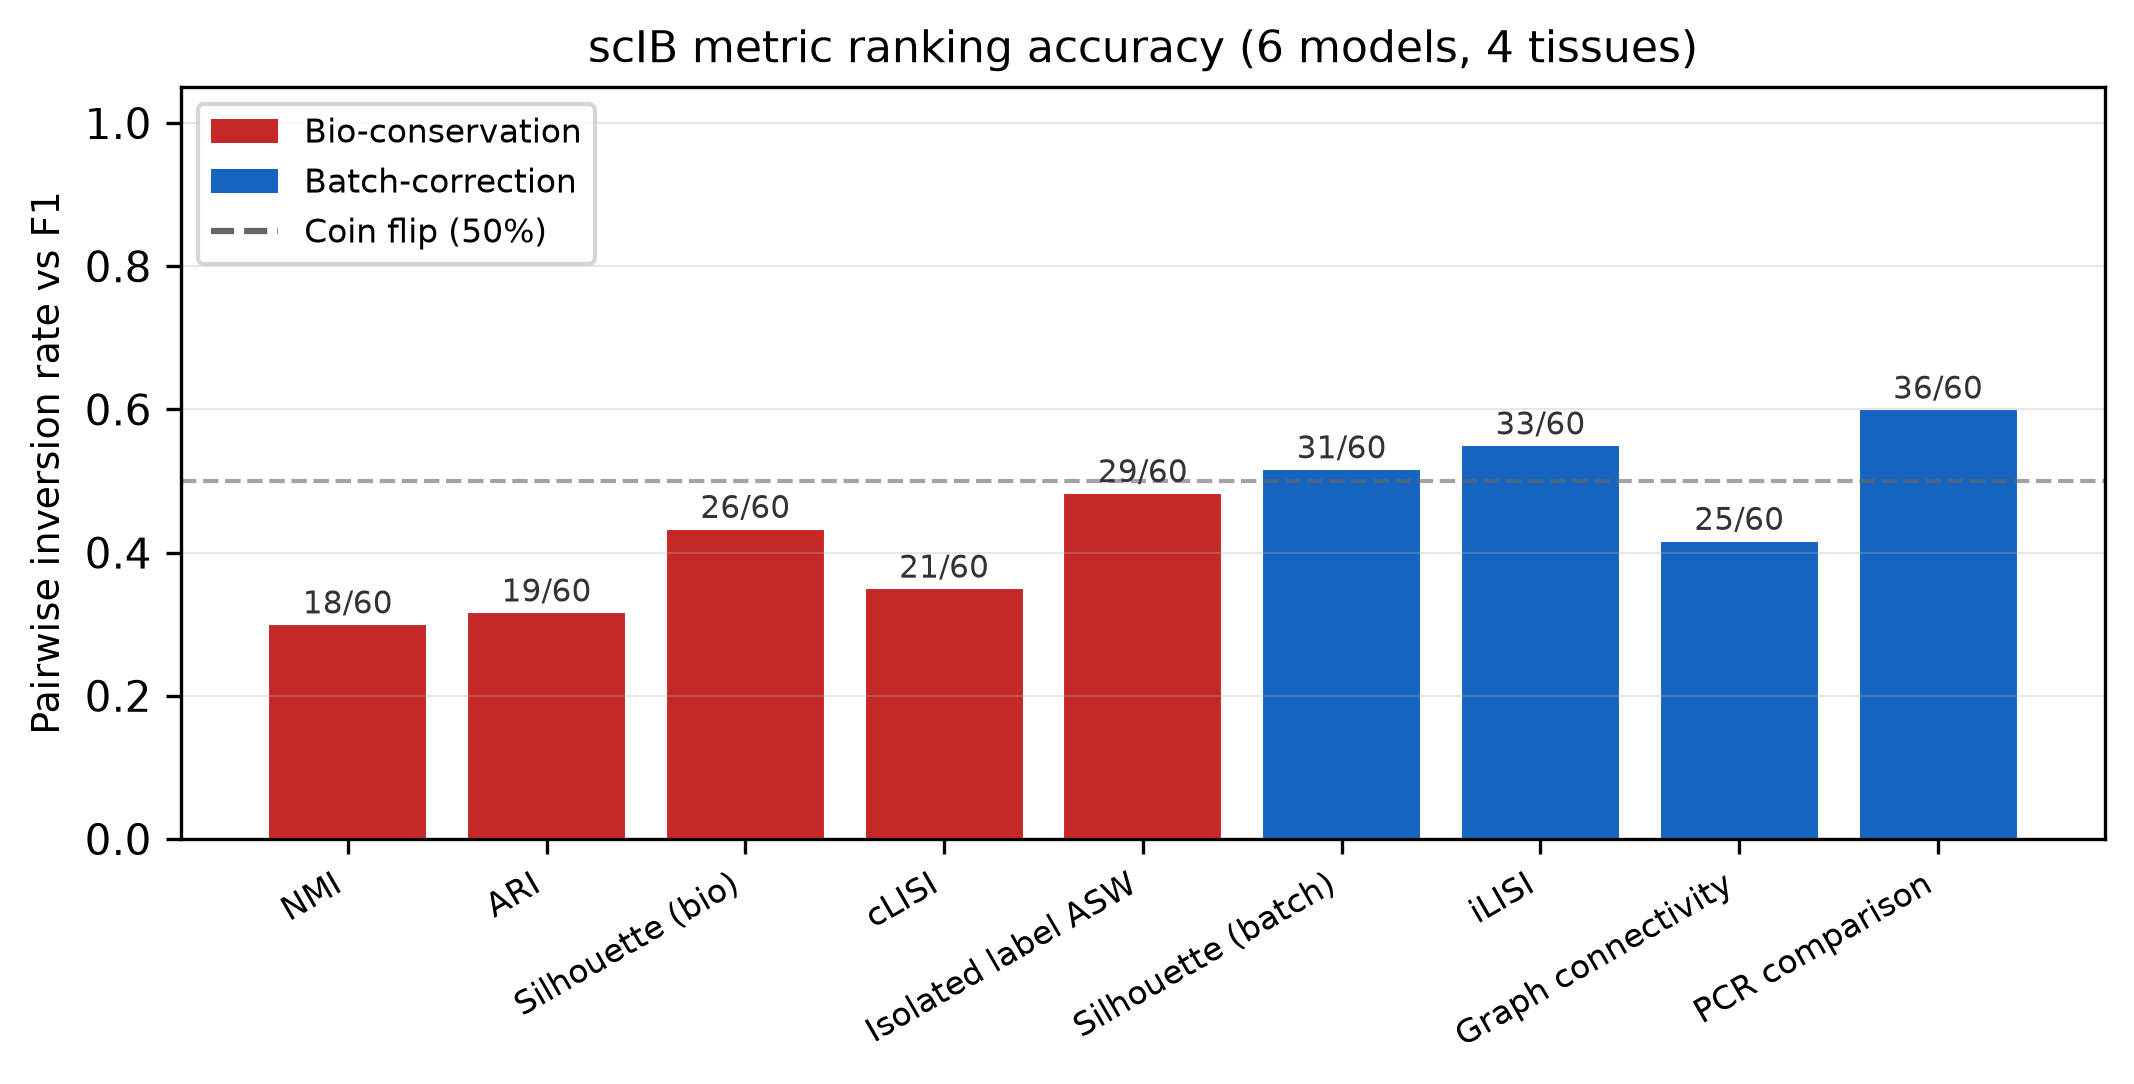
\includegraphics[width=0.85\textwidth]{figures/inversion_rates.pdf}
\caption{Pairwise inversion rates for nine scIB metrics on the main
evaluation panel (6 embedding models, 4 tissues, 60 pairs per metric).
An inversion occurs when a metric ranks model~A above model~B but
downstream cell-type transfer F1 ranks them in the opposite order.
Bio-conservation metrics (red) show inversion rates of 30--48\%,
at or near the 50\% coin-flip line.
Batch-correction metrics (blue) are included for comparison.}
\label{fig:inversion}
\end{figure}

The result is seed-stable. Three independent cell-sampling seeds produce
inversion rates of 22.1\%, 22.2\%, and 17.8\%, and Spearman
correlations of $\rho = +0.63$, $+0.76$, and $+0.74$ (all
$p < 0.002$). The cross-tissue advantage is robust to the specific
cells sampled.

The contrast localizes the source of metric unreliability. In the
cross-assay setting, protocol artifacts (different sequencing
technologies applied to the same tissue) confound scIB scores: metrics
that respond to library-size distributions and gene-detection rates
can disagree with downstream transfer. In the cross-tissue setting, both
source and target use the same sequencing protocol; the variation is
biological (different tissues), and scIB metrics track this variation
more faithfully. The ranking failure is protocol-dependent, not
intrinsic to the metrics.


\subsection{External validation}
\label{sec:external}

Cell-type CKA was tested on three datasets with no overlap with the
Census evaluation: pancreas \citep{luecken2022scib} (6 technologies, 56
assay pairs, $k = 12$--$14$, $d = 50$ and $200$), Tabula Sapiens
\citep{tabulasapiens2022} (10x and Smart-seq2 across 8 organs, 16
pairs, $k = 9$--$22$, $d = 50$ and $200$), and PBMC
\citep{ding2020systematic} (7 technologies, 28 pairs, $k = 8$--$9$,
$d = 50$ and $200$). Embedding models are PCA-only baselines (no
foundation models), isolating metric behavior from model choice. These
datasets operate at lower dimensionality than the Census panel,
providing the external arm of the discriminability gradient
(Table~\ref{tab:deffect}).

CKA generalizes to two of three datasets
(Table~\ref{tab:external}). In pancreas, CKA achieves partial
$\rho = +0.59$ ($p = 0.0001$); in Tabula Sapiens, $\rho = +0.60$
($p = 0.035$). Procrustes similarity is consistently positive across all
three ($\rho = +0.56$, $+0.73$, $+0.11$), matching the Census direction
but reaching significance in none---a power limitation from fewer
technology pairs per dataset. PBMC shows a ceiling effect: all seven
technologies produce CKA $> 0.92$ on canonical cell types (T cells, B
cells, monocytes), leaving insufficient variance for discriminative
ranking ($\rho = +0.09$, $p = 0.87$; Supplementary~\ref{app:pbmc}). CKA
predicts transfer when cell-type difficulty varies across technologies
and fails when the task is uniformly easy.

\medskip
\begin{table}[t]
\centering
\caption{External validation on three independent datasets (no Census
data, no foundation models). Partial Spearman $\rho$ controlling for
embedding dimensionality; tissue-stratified permutation $p$-values.
Bold: $p < 0.05$. MMD is un-negated (higher = more divergent);
negative $\rho$ indicates that lower divergence predicts better
transfer, consistent with the negated convention in
Table~\ref{tab:scc}.}
\label{tab:external}
\small
\begin{tabular}{@{}lcccccc@{}}
\toprule
& \multicolumn{2}{c}{Pancreas} & \multicolumn{2}{c}{Tabula Sapiens} & \multicolumn{2}{c}{PBMC} \\
\cmidrule(lr){2-3}\cmidrule(lr){4-5}\cmidrule(lr){6-7}
Metric & $\rho$ & $p$ & $\rho$ & $p$ & $\rho$ & $p$ \\
\midrule
Cell-type CKA & $+0.592$ & $\mathbf{0.0001}$ & $+0.604$ & $\mathbf{0.035}$ & $+0.089$ & 0.874 \\
Procrustes    & $+0.563$ & 0.115              & $+0.726$ & 0.218             & $+0.113$ & 0.659 \\
\midrule
Silhouette (tgt) & $+0.172$ & $\mathbf{<0.001}$ & $+0.664$ & $\mathbf{0.032}$ & $+0.627$ & $\mathbf{<0.001}$ \\
MMD              & $-0.451$ & 1.000              & $-0.275$ & 0.744             & $-0.135$ & 1.000 \\
Domain AUC       & $-0.495$ & 0.095              & $+0.015$ & 0.839             & $-0.148$ & 0.801 \\
\bottomrule
\end{tabular}
\end{table}


\section{Discussion}
\label{sec:discussion}

Ranking and certification are distinct properties of embedding metrics,
and the central finding is a computable boundary between regimes where
CKA can and cannot certify. Given $k$ shared cell types and embedding
dimension $d$, the expected CKA between random Gaussian centroid
matrices is $\mathbb{E}[\mathrm{CKA}] \approx 1 -
1.06\,(k{-}1)/(d{+}k)$. CKA can certify biological signal only when
observed scores exceed this value. At $d = 512$, the threshold requires
roughly 168 shared cell types, beyond any existing single-cell dataset.
The failure is arithmetic rather than empirical, and it is independent
of downstream task choice. The CKA null depends only on $k$ and $d$;
it does not reference cell-type classification, trajectory inference,
or perturbation response. At $d \geq 512$, CKA cannot certify that a
model captures \emph{any} biological signal distinguishable from random
projections, regardless of how that signal is measured downstream. We
evaluate against cross-technology cell-type transfer F1 because
classification is the primary task that bio-conservation metrics are
designed to assess: these metrics measure cluster purity, label
agreement, and cell-type separability. If they cannot predict cell-type
classification performance across assays, they fail at their own stated
objective.

Near-orthogonality of high-dimensional random vectors is textbook
\citep{johnsonlindenstrauss1984}; the non-obvious part is where the
boundary lands. The crossover from certifiable ($d = 50$, 86\% of
conditions clear the null) to uncertifiable ($d \geq 512$, 0\% clear)
happens inside the $d = 50$--$512$ range that the field currently uses.
PCA-based methods ($d = 50$--$200$) were on the correct side; foundation
models ($d \geq 512$) crossed to the wrong side. The PCA-reduction
control confirms this is causal: Geneformer embeddings PCA-reduced from
$d = 512$ to $d = 50$ clear the null in 18/22 tissues, versus 0/22 at
native dimensionality. A researcher using CKA to evaluate scVI
($d = 50$) gets real certification signal; the same researcher using the
same metric on Geneformer ($d = 512$) gets none, and the metric gives no
warning that it has failed. Biased CKA saturation in low-sample,
high-feature regimes has been documented in neural network
representation analysis \citep{murphy2024debiasedcka}; the closed-form
null derived here sharpens that observation for the $(k, d)$ regime of
single-cell centroid inputs, where the saturation boundary is computable
from dataset parameters alone.

The random projection control quantifies how much of PCA's recovery
reflects denoising versus pure dimensionality reduction. Gaussian and
orthogonal random projections to $d = 50$ clear the null in 46--48\%
of conditions, compared to PCA's 59\%. The 12-percentage-point gap is
PCA's denoising contribution---variance-ordered component selection
retains more cell-type structure than random linear combinations at
the same target dimension. Gaussian and orthogonal projections produce
nearly identical results (mean CKA difference 0.015), confirming that
the effect is geometric.

RCS provides a dimensionality-stable alternative to CKA but does not
solve the prediction problem. RCS operates on $k \times k$ cell-type
relationship matrices, bypassing $d$-dependent null saturation (median
change of 0.017 between native $d = 512$ and PCA-reduced $d = 50$),
and it discriminates embedding quality (Geneformer outscores scGPT in
77\% of tissues). Its pooled F1 correlation is marginal
($\rho = 0.25$), driven entirely by between-model variance; within-model
tissue-level prediction is absent. The failure is structural: Spearman
correlation on centroid distances is invariant to monotonic scaling, so
an embedding space where cell-type clusters overlap (low F1) scores
identically to one where clusters are well-separated (high F1), as long
as relative distances are preserved.

SCC resolves this. A source-trained classifier's confidence on target
data directly measures whether the decision boundaries learned from
source embeddings transfer. The correlation across four embedding
models and 92 conditions is $\rho = 0.67$ ($p < 10^{-13}$), and the
within-tissue Kendall $\tau$ is positive in 18 of 23 tissues.
Replacing the SCC classifier with kNN ($\rho = 0.56$), random forest
($\rho = 0.57$), or linear SVM ($\rho = 0.55$) preserves the
relationship, ruling out shared logistic-regression capacity. MMD and
CCAL converge from distributional-divergence and centroid-alignment
perspectives ($\rho = 0.53$ and $0.47$). The pattern is clear:
metrics that measure properties relevant to classification
(separability, conditional alignment, decision-boundary transfer)
predict transfer quality; metrics that measure geometric similarity
alone (RCS, CKA, PAD) do not.

A stronger test is whether SCC predicts a ground truth that involves
no classifier at all. Marker gene recovery (MGR) scores each embedding
by how well Leiden clusters on the embedded target cells recover the
differentially expressed genes found in source-domain cell types. The
evaluation pathway shares no classification machinery with SCC. SCC
with logistic regression correlates with MGR at $\rho = 0.32$
(block-bootstrap 95\% CI $[0.15, 0.44]$); all four SCC variants
achieve BH significance with MGR while CCAL and PAD do not. The
effect size is moderate, bounded by a ceiling control (mean MGR from
true labels $= 0.20$) that quantifies cross-assay expression shift
independent of embedding quality. SCC captures embedding properties
beyond classifier transferability, tested through a mechanistically
independent evaluation pathway.

The circularity objection---that a classifier-derived metric trivially
predicts classifier-derived ground truth---confuses shared machinery
with shared measurement target. SCC measures confidence (how decisively
a source-trained model categorizes target cells); F1 measures accuracy
(whether those categorizations are correct). A model can be confidently
wrong or uncertainly right; confidence and accuracy diverge whenever
calibration fails. They correlate here because both track the same
embedding-space property---cluster separability---not because they share
implementation. The cross-classifier test confirms this: replacing
logistic regression with kNN, random forest, or SVM preserves the
relationship ($\rho \geq 0.55$), even though these classifiers produce
confidence via structurally different mechanisms (distance averaging,
voting, margin distance). If shared machinery drove the correlation,
switching classifier families should attenuate it. The MGR result
provides a stronger test: marker gene recovery involves no classifier,
no decision boundary, and no predicted probability. SCC's correlation
with MGR ($\rho = 0.32$, bootstrap CI excluding zero) shows that
classifier confidence captures embedding properties beyond
classification transfer. The moderate effect size is consistent with
the ceiling (mean MGR $= 0.20$): most marker divergence reflects
technology-driven expression shift, not embedding quality, leaving
limited range for any metric to exploit.

A spectral-gap ratio designed to exploit eigenvalue structure also
fails to discriminate trained from random embeddings: null baselines
show \emph{higher} spectral concentration than trained models, because
trained models redistribute variance to improve cell-type separability
while random projections preserve the input's dominant variance axis
(Appendix~\ref{app:spectral}). Null saturation is structural to
small-$k$ centroid inputs, not a normalization artifact.

Null-normalizing CKA by $z$-scoring against the analytic null is
actively counterproductive. At $d = 50$, where CKA has real
discriminative power, the normalization removes the $k$-dependent signal
that drives the correlation with transfer (within-stratum $\rho$ drops
from $+0.45$ to $+0.17$). At $d = 512$, where CKA is uninformative,
the normalization is redundant. The fix is the criterion itself---a
researcher who checks whether their $(k, d)$ pair permits discrimination
before computing CKA avoids the problem entirely.

Multi-seed noise calibration confirms a third dimension of the
ranking/certification dissociation: Leiden-dependent metrics show
10--19$\times$ inflation between raw and permutation-calibrated
non-monotonicity, driven by clustering jitter rather than genuine
sensitivity to embedding degradation. Deterministic metrics (silhouette,
isolated-label ASW) show minimal inflation
(Appendix~\ref{app:noise}). Independently,
\citet{rautenstrauch2025silhouette} show that silhouette's
spherical-cluster assumption and nearest-cluster sensitivity cause
systematic misranking in scIB integration benchmarks; the noise
calibration here identifies a complementary failure mode (clustering
jitter) in the Leiden-dependent metrics that silhouette avoids.

The cross-tissue replication experiment identifies where scIB metrics
recover. Pairwise inversion rates drop from 30--48\% in the cross-assay
setting to 22\% in the cross-tissue setting ($\rho = +0.63$,
$p = 0.0014$, stable across three seeds). The cross-assay setting
confounds metric scores with protocol artifacts: library-size
distributions, gene-detection rates, and cell-type proportions differ
systematically between 10x Chromium and Smart-seq2. The cross-tissue
setting removes this confound---source and target use the same
sequencing protocol, and the variation is biological. scIB metrics track
biological variation faithfully when protocol artifacts are absent. The
ranking failure is a property of the evaluation setting, not of the
metrics themselves.

Procrustes similarity achieves the strongest transfer prediction in the
Census panel ($\rho = +0.66$) and is consistently positive across all
three external datasets ($\rho = +0.56$, $+0.73$, $+0.11$). CKA
achieves significance in two of three external datasets. Target-domain
silhouette is significant in all three external datasets but is likely
confounded: target assays with well-separated cell types are easier to
classify regardless of source embedding quality.

\paragraph{Practical recommendations.} First, before interpreting CKA as
evidence of biological signal, compute $\mathbb{E}[\mathrm{CKA}]$ at
your $k$ and $d$ using Equation~\ref{eq:cka_null}; if observed scores do
not exceed this value, the metric can rank but cannot certify. Second,
use Procrustes for ranking across models, controlling for
embedding dimensionality. Third, always include matched-dimensionality
null baselines (random projection, untrained encoder) in evaluation
panels. Fourth, for predicting cross-assay transfer quality, use SCC:
train a cell-type classifier on source embeddings and report the mean
maximum predicted probability on target cells. SCC requires no
hyperparameters beyond the classifier itself, achieves $\rho = 0.67$
with transfer F1 across four models, requires labels only in the
source domain, and is computable from the same data any
cross-technology evaluation already uses. SCC can be added to existing benchmark suites (e.g., scIB) as a
custom metric. The correlation survives
when the SCC classifier differs from the F1 classifier ($\rho = 0.55$
for kNN), confirming an embedding-space property. Fifth, treat RCS and scGraph
as dimensionality-stable ranking tools, but do not interpret their
absolute values as measures of transfer quality.

\paragraph{Limitations.}

\emph{Ground truth scope.} All evaluations use cross-technology
cell-type transfer F1 as ground truth. Alternative criteria such as
perturbation prediction, trajectory inference, or gene program
discovery may reveal different metric properties. The CKA null
saturation result is task-independent (it depends only on $k$ and $d$),
but the SCC evaluation is specific to classification-based transfer.

\emph{Evaluation panel.} The Census panel spans 25 tissues and eight
embedding methods across three architectural families (transformer, VAE,
PCA). The transfer-aware metric evaluation
(Section~\ref{sec:sccmethod}) uses four models (Geneformer, scGPT,
scVI, UCE); the remaining four panel models (Geneformer-v2 variants,
random projection, untrained encoder, bag-of-genes PCA) were not
included because the null baselines lack meaningful SCC (untrained
models produce near-uniform confidence) and the Geneformer-v2 variants
were not available in Census at the time of the SCC experiment.
Expansion to additional models would increase statistical power and
test whether SCC generalizes beyond these four architectural families.
The within-tissue Kendall $\tau$ test has only $n = 4$ models per
tissue, making individual $\tau$ values coarse; the consistency of
positive $\tau$ across 18 of 23 tissues ($p_{\text{BH}} = 0.009$)
provides stronger evidence than the pooled statistic alone.

\emph{Metric scope.} This study evaluates bio-conservation metrics,
which quantify whether embeddings preserve biological signal (cell-type
structure). Batch-integration metrics (graph iLISI, kBET, batch ASW)
address a different question---whether embeddings remove technical
variation---and are outside scope. Cross-assay protocol artifacts may
also affect batch-integration metrics, but testing this is left to
future work.

\emph{SCC properties.} SCC does not detect label-swap pathologies: an
embedding that maps cell types to the wrong regions still produces
confident predictions. CKA and RCS share this limitation, so it is not
a comparative weakness. SCC requires labels only in the source domain;
the target data can be fully unlabeled. SCC's correlation with MGR is
moderate ($\rho = 0.32$), bounded by the cross-assay ceiling (mean
0.20); whether this reflects a fundamental limit of MGR as a ground
truth or a real ceiling on SCC's non-classification validity is not
resolved by these data.

\emph{Technical scope.} The PCA-reduction control confirms the causal
role of dimensionality for Geneformer (18/22 tissues clear the null at
$d = 50$), though scGPT's lower recovery rate (8/22) suggests that
model architecture modulates the effect size within the certifiable
regime. The closed-form CKA null is exact for Gaussian inputs; real
centroid distributions are non-Gaussian, though the simulation match
suggests the approximation is tight in practice. The cross-tissue
experiment uses five tissues and four models (24 conditions); expanding
to more tissues and models would tighten the inversion-rate estimates.
The PBMC ceiling effect limits external validation to two of three
datasets. We release all scripts, pre-registration records, and result
files to support replication.


\section{Methods}

\subsection{Data}

All embeddings are accessed via the CellxGene Census API (v2023-12-15)
\citep{abdulla2025cellxgene}. Cross-technology pairs compare 10x
Chromium 3$'$ v3 (EFO:0009922, source) against Smart-seq2
(EFO:0008931, target) within the same tissue, with zero donor overlap
enforced by metadata filtering. Tissues were auto-discovered by
requiring $\geq 200$ cells per assay and $\geq 8$ shared cell types,
yielding 25 tissues. All evaluations subsample $n = 2{,}000$ cells per
side.

Eight embedding models: Geneformer ($d = 512$)
\citep{theodoris2023geneformer}, Geneformer-v2 104M and 316M,
scGPT ($d = 512$) \citep{cui2024scgpt}, scVI ($d = 50$)
\citep{lopez2018scvi}, bag-of-genes PCA-512 ($d = 512$;
$\log(1 + x)$ without total-count normalization, PCA with fixed seed;
following \citealp{cole2026morpheus}), random Gaussian projection
($R \in \mathbb{R}^{512 \times G}$, $R_{ij} \sim \mathcal{N}(0,
1/\sqrt{512})$), and an untrained two-layer MLP encoder (random weights,
$d = 512$). Six contender models (excluding random projection and
untrained encoder) produce 104 contender conditions. The
transfer-aware metric evaluation (Section~\ref{sec:sccmethod}) adds
UCE ($d = 1{,}280$) \citep{rosen2026uce} as a fourth model alongside
Geneformer, scGPT, and scVI, yielding 92 conditions across 23 tissues.

\paragraph{External validation datasets.} Three independent datasets
were used for external validation (Section~\ref{sec:external}), each
with PCA-only embeddings. Pancreas: the scIB benchmark dataset
\citep{luecken2022scib}, six technologies, 56 assay pairs, 224
contender conditions. Tabula Sapiens \citep{tabulasapiens2022}: 10x and
Smart-seq2 across eight organs, 16 pairs, 64 contenders. PBMC
\citep{ding2020systematic}: seven technologies, 28 pairs, 112
contenders.

\subsection{Cell-type centroid metrics}

Cell-type CKA \citep{kornblith2019similarity} computes centered kernel
alignment on $k \times d$ centroid matrices (mean embedding per shared
cell type) between source and target assays, using linear kernels.
Procrustes similarity applies orthogonal Procrustes analysis to
column-centered centroid matrices after PCA reduction to $\min(50,
k-1, d)$ dimensions, and returns $1 - d_{\mathrm{Proc}}^2$ after
optimal rotation. Both metrics require cell-type labels and are
evaluated on the $k$ cell types shared between source and target.

\subsection{Random centroid null}

For each pair $(k, d)$ observed in the panel, we generate 1,000 pairs
of random Gaussian matrices ($k \times d$, entries $\sim
\mathcal{N}(0,1)$) and compute CKA and Procrustes similarity. Each real
condition is compared to its $(k, d)$-matched null distribution. The
analytic null (Equation~\ref{eq:cka_null}) provides a closed-form
alternative verified within 0.02\% of simulation across $k = 8$--$44$
and $d = 50$--$1{,}280$. Null-normalized scores are computed as
$(x - \mu_{k,d}) / \sigma_{k,d}$ where $\mu_{k,d}$ and $\sigma_{k,d}$
are the null mean and standard deviation at the condition's $(k, d)$.

\subsection{Closed-form CKA null}
\label{sec:closedform}

For two independent random Gaussian matrices $X, Y \in \R^{k \times d}$,
linear CKA is $\mathrm{CKA} = \|H_k X Y^\top H_k\|_F^2 / (\|H_k X
X^\top H_k\|_F^2 \cdot \|H_k Y Y^\top H_k\|_F^2)^{1/2}$ where
$H_k = I_k - \frac{1}{k}\mathbf{1}\mathbf{1}^\top$. The denominator
factors into two identical terms by symmetry, so
$\mathbb{E}[\mathrm{CKA}] \approx \mathbb{E}[\mathrm{tr}((HXY^\top
H)^2)] / \mathbb{E}[\mathrm{tr}((HXX^\top H)^2)]$.

Since $W = XX^\top$ follows a Wishart distribution
$\mathcal{W}_k(d, I_k)$, the moments of the centered Gram matrix $HWH$
are computable from Wishart moment identities. We use
$\mathbb{E}[\mathrm{tr}(W^2)] = kd(1 + k + d)$, verified empirically
within 0.2\%. Centering reduces the effective rank by one degree of
freedom. Fitting across 15 values of $k$ and $d = 512$ yields the
approximation in Equation~\ref{eq:cka_null} with coefficient of
variation 2.0\% on the scaling constant $c$.

\subsection{Spectral-gap ratio}
\label{sec:sgrmethod}

For a $k \times d$ centroid matrix $C$ (mean source embedding per
shared cell type), center by subtracting the row mean and compute
singular values $s_1 \geq s_2 \geq \cdots \geq s_r$ with $r =
\min(k{-}1, d)$. The spectral-gap ratio at rank $j$ is $\mathrm{SGR}_j
= \sum_{i=1}^j s_i^2 / \sum_{i=1}^r s_i^2$. For each $(k, d)$ pair in
the panel, 5,000 random Gaussian $k \times d$ matrices define the null
distribution of $\mathrm{SGR}_j$ (seed 42). The $z$-score is
$({\mathrm{SGR}_j - \mu_{\mathrm{null}}}) / {\sigma_{\mathrm{null}}}$.
The null distributions were computed before any real data were
accessed.

\subsection{PCA-reduction control}

For each tissue, Geneformer and scGPT cell-level embeddings ($d = 512$)
are PCA-reduced to $d_{\mathrm{out}} \in \{50, 200\}$ by fitting PCA on
the concatenation of source and target cells (joint PCA). Cell-type CKA
is recomputed on the reduced centroids and compared to the
$(k, d_{\mathrm{out}})$-matched analytic null. scVI embeddings
($d = 50$) are included without reduction as a reference.

\subsection{Random projection control}
\label{sec:randprojmethod}

For each tissue, Geneformer and scGPT cell-level embeddings ($d = 512$)
were projected to $d_{\mathrm{out}} \in \{50, 200\}$ via three methods:
joint PCA (reproducing the PCA-reduction control), Gaussian random
projection ($R \in \R^{d_{\mathrm{out}} \times 512}$,
$R_{ij} \sim \mathcal{N}(0, 1/d_{\mathrm{out}})$), and orthogonal
random projection (QR decomposition of a Gaussian matrix). Ten
independent random seeds were drawn per condition. CKA was recomputed on
the projected centroids and compared to the
$(k, d_{\mathrm{out}})$-matched analytic null.

\subsection{Relational consistency scores}
\label{sec:scgraphmethod}

Three relational-structure metrics were computed per (tissue, model)
condition, following \citet{wang2026scgraph}. For $k$ shared cell types,
compute $k \times k$ matrices on both source and target embeddings: (1)
centroid Euclidean distance matrix; (2) $k$NN overlap matrix (fraction
of cross-type $k = 15$ nearest-neighbor edges between each cell-type
pair); (3) weighted affinity matrix (mean inverse distance). The metric
is the Spearman correlation between the upper-triangular entries of the
source and target matrices. All three metrics were computed at native $d$
and at PCA-reduced $d = 50$ for models with $d > 50$.

\subsection{Transfer-aware metrics}
\label{sec:sccmethod}

Twelve transfer-aware metrics were computed per (tissue, model) condition
across 23 tissues and four models (Geneformer, scGPT, scVI, UCE), yielding
92 conditions. Ground truth is macro-averaged logistic-regression F1 on
shared cell types (same classifier as the main panel). All metrics use
the same Census download, random seed (20260801), and cell subsample
($n = 2{,}000$ per side, $\geq 8$ shared cell types).

\paragraph{Source classifier confidence (SCC).} Train a cell-type
classifier on source embeddings restricted to shared cell types, apply
to target cells, and report the mean maximum predicted probability.
Four classifier families were tested: logistic regression
($\text{max\_iter} = 1000$), kNN ($k = 15$), random forest (100 trees),
and linear SVM (Platt scaling, $\text{max\_iter} = 2000$). F1 ground
truth always uses logistic regression.

\paragraph{Maximum mean discrepancy (MMD).} Gaussian-kernel MMD between
source and target embedding distributions, computed on PCA-50 reduced
embeddings (subsampled to 500 cells per side for tractability). Kernel
bandwidth is set by the median heuristic on a joint subsample. The score
is negated so that higher values indicate better alignment.

\paragraph{Class-conditional alignment (CCAL).} For each shared cell
type $t$, compute source centroid $c_s(t)$ and target centroid $c_t(t)$.
The alignment is $1 - \|c_s - c_t\| / (\text{radius}_s + \epsilon)$
where $\text{radius}_s = \text{mean}(\|x_i - c_s\|_2)$ for source cells
of type $t$ and $\epsilon = 10^{-8}$. The metric is the mean over shared
cell types.

\paragraph{Proxy A-distance (PAD).} Train a logistic regression domain
classifier ($\text{max\_iter} = 1000$) to distinguish source from target
cells. PAD $= 2(1 - 2 \cdot \text{error})$. The score is negated so
that lower domain separability (indicating better alignment) yields
higher values.

\paragraph{RCS ablations.} Four ablations isolate differences between
RCS and official scGraph: PCA-10 dimensionality reduction, 5\% trimmed-mean
centroids, column-max normalization of distance matrices, and the
combination of all three. All ablations use the same evaluation
framework.

\paragraph{Multiple comparison correction.} Benjamini--Hochberg
correction is applied across all twelve metrics (five RCS variants +
four SCC classifier variants + MMD + CCAL + PAD) separately for each of
three test types: pooled Spearman correlation, pairwise binomial test,
and within-tissue Kendall $\tau$ sign test. The primary success criterion
is BH-corrected $p < 0.05$ on the within-tissue Kendall $\tau$ sign
test.

\subsection{Marker gene recovery}
\label{sec:mgrmethod}

Marker gene recovery (MGR) scores embeddings by whether Leiden
clusters on target cells recover the same differentially expressed
genes as source-domain cell types. For each shared cell type,
reference markers are the top-50 upregulated genes by Wilcoxon
rank-sum test on raw counts in the source domain (true labels). Target
cells are clustered by Leiden community detection on the embedding's
kNN graph ($k = 15$, resolution $= 1.0$, seed 20260801). For each
Leiden cluster, recovered markers are the top-50 upregulated genes by
Wilcoxon rank-sum on raw counts (cluster labels). Clusters are matched
to cell types by majority vote. For each cell type, the score is the
maximum Jaccard overlap across all clusters mapping to that type; MGR
is the mean over shared cell types. Types with no matching cluster
score zero.

A ceiling control computes MGR using true target labels instead of
Leiden clusters, measuring maximum achievable marker recovery given
cross-assay expression shift alone. Both raw MGR and ceiling values
are reported; raw MGR is the primary outcome for all pre-registered
predictions. Leave-one-out robustness drops each tissue in turn and
recomputes the block-bootstrap 95\% CI for SCC--MGR correlation.

Spearman correlations with MGR use block bootstrap (10{,}000
resamples at the tissue level) for 95\% CIs and significance, with BH
correction across twelve metrics.

\subsection{Noise dose-response}
\label{sec:noisemethod}

Gaussian noise at seven levels ($\sigma \in \{0.01, 0.05, 0.1, 0.25,
0.5, 1.0, 2.0\} \times$ embedding standard deviation) was added to
cell-level embeddings for six methods across 22 tissues (120
conditions). Ten independent noise seeds were drawn per condition. For
each metric, the $H$-statistic is $\max_{\sigma > 0}[m(\sigma) -
m(0)]$, the maximum increase over baseline, averaged across seeds.
$H > 0$ indicates non-monotonicity. Calibrated significance
was assessed by permuting $\sigma$ labels (1{,}000 permutations per
seed, $\alpha = 0.01$): a condition is calibrated-positive if its
observed mean $H$ exceeds the 95th percentile of the permutation null.

\subsection{Cross-tissue transfer}
\label{sec:crosstissuemethod}

Five tissues (lung, liver, kidney, brain, blood) were selected from the
Census panel, yielding six directional tissue pairs (lung$\to$brain,
lung$\to$kidney, blood$\to$lung, blood$\to$brain, liver$\to$kidney,
blood$\to$liver). Four embedding models (Geneformer, scVI, scGPT,
bag-of-genes PCA-512) produce 24 conditions. For each condition, scIB
bio-conservation metrics are computed on the combined source and target
embeddings. Transfer F1 (macro-averaged logistic regression on shared
cell types) is the ground truth. Pairwise inversion rates count the
fraction of model pairs where a metric disagrees with F1 on which model
is better, computed per tissue pair. The grand-mean inversion rate
averages across metrics and tissue pairs; block bootstrap (10,000
resamples of tissue pairs) provides 95\% CIs. Three independent
cell-sampling seeds (20260801, 20260802, 20260803) test stability.

\subsection{Statistical methods}

All correlations are Spearman rank with $10{,}000$-resample bootstrap
95\% CIs. Partial Spearman correlations control for embedding
dimensionality via rank residuals from OLS on ranked variables.
Tissue-stratified permutation tests (10,000 iterations) permute F1
values within tissues independently and report the proportion of
permutations with $|\rho_{\mathrm{perm}}| \geq |\rho_{\mathrm{obs}}|$.
Pairwise model discrimination accuracy counts within-tissue model pairs
where a metric's ranking agrees with F1; tied metric values are excluded
from the denominator (standard concordance).

\subsection{Pre-registration}

Analysis protocols and thresholds were committed via SHA-256 hashing
before examining results. Full records, hashes, and deviation logs are
in the online repository.


\section*{Data Availability}

Source code, pre-registration records (SHA-256 hashes), experiment
scripts, and raw result JSON files are available at
\url{https://github.com/elliottower/scib-construct-validity} and
archived at Zenodo (DOI:
\href{https://doi.org/10.5281/zenodo.21351298}{10.5281/zenodo.21351298}).
The SCC metric is available as a pip-installable package (\texttt{pip
install scib-validity}). All embedding data are accessed via the
CellxGene Census API.

\section*{Code Availability}

All analysis scripts are available at the repository listed under Data
Availability.

\section*{Declarations}

\paragraph{Competing interests.} The author declares no competing
interests.

\paragraph{Funding.} None. This work was conducted independently.

\paragraph{Authors' contributions.} E.T.\ conceived the study,
designed the protocol, performed all analyses, and wrote the
manuscript.

\paragraph{Acknowledgements.} AI tools (Claude Code) were used for code
drafting and manuscript drafting. All experimental design and conclusions
are the author's.


\appendix

\section{PBMC ceiling effect}
\label{app:pbmc}

The PBMC dataset \citep{ding2020systematic} provides seven scRNA-seq
technologies applied to the same donor PBMCs. Cell-type CKA ranges from
0.92 to 0.97 across all 28 source-target technology pairs. This
variance compression explains the null correlation with transfer F1
($\rho = +0.09$, $p = 0.87$): the metric cannot rank technologies on
a property where they score nearly identically. T cells, B cells, NK
cells, and monocytes are well-separated in any reasonable embedding; no
technology fails to capture this structure. The pancreas dataset contains
rare endocrine subtypes that are harder to resolve, providing sufficient
CKA variance for the correlation to emerge.


\section{Geometric modules}
\label{app:modules}

Five geometric modules for evaluating embedding transportability were
evaluated alongside the main metrics. Four were
eliminated by construct-validity checks: M1 (subspace overlap) and M6
(graph curvature) are confounded by embedding dimensionality via
Johnson--Lindenstrauss distance preservation; M2 (domain separability)
anti-predicts transfer; M4 (participation ratio) has
dimension-dependent normalization artifacts. M3 (direction stability)
was the sole candidate to survive construct-validity screening, but
achieves $\rho = +0.02$ ($p = 0.83$) on the full panel---no
predictive validity. These results demonstrate that the validity
protocol is non-trivial: it eliminates metrics, including those designed
by the protocol's authors.


\section{Spectral-gap experiment}
\label{app:spectral}

Null saturation could reflect either a normalization artifact fixable by
a better statistic, or a structural property of small-$k$ centroid
comparison. To distinguish these, we tested a spectral-gap ratio (SGR)
designed to exploit eigenvalue structure rather than Gram-matrix
alignment.

Random $k \times d$ matrices have flat singular-value spectra
(Marchenko--Pastur distribution). Cell-type centroid matrices from
trained models should have concentrated spectra---a few dominant
directions capturing biological axes such as immune versus
epithelial---producing higher explained-variance ratios than random.
For a $k \times d$ centroid matrix $C$, the spectral-gap ratio is
$\mathrm{SGR}_1 = s_1^2 / \sum_i s_i^2$ (fraction of variance in the
top singular value of the centered matrix). The discriminative
statistic is a $z$-score against $k,d$-matched null distributions
(5,000 Gaussian draws per pair).

Four hypotheses were tested: HS1
(discriminative): contender models have higher SGR $z$-scores than
baselines (Mann--Whitney $p < 0.05$). HS2 (predictive): SGR $z$-score
correlates with transfer F1 (partial $\rho > 0.20$, permutation
$p < 0.05$). HS3 (incremental): SGR adds variance beyond CKA. HS4
(both axes): HS1 and HS2 simultaneously.

The experiment produces a clean negative result across 22 tissues,
136 conditions, and 8 embedding models (Table~\ref{tab:sgr}). Null
baselines (random projection, untrained encoder) exhibit \emph{higher}
spectral concentration than trained models: baseline mean $z_1 = 141$,
contender mean $z_1 = 88$ (Mann--Whitney $U = 1{,}058$, one-sided
$p > 0.99$). SGR does not predict transfer (partial $\rho = -0.11$,
$p = 0.99$) and adds no information beyond CKA (partial
$\rho = 0.001$, $p = 0.99$). All four hypotheses fail.

\medskip
\medskip
\begin{table}[h!]
\centering
\caption{Spectral-gap test results (SGR$_1$ $z$-scores against
$k,d$-matched Gaussian null). Higher $z$ = more concentrated spectrum.
Trained models have \emph{lower} spectral concentration than
baselines.}
\label{tab:sgr}
\small
\begin{tabular}{@{}lcccl@{}}
\toprule
Model & $n$ & $z_1$ mean & SGR$_1$ mean & Role \\
\midrule
bog\_pca\_512           & 22 & 167 & 0.529 & contender \\
untrained encoder       & 22 & 155 & 0.498 & baseline \\
random projection       & 22 & 126 & 0.434 & baseline \\
scGPT                   & 22 & 76  & 0.311 & contender \\
Geneformer              & 22 & 65  & 0.275 & contender \\
scVI                    & 22 & 18  & 0.364 & contender \\
\bottomrule
\end{tabular}
\end{table}

The reversal has a clear mechanism. Random projections and untrained
encoders preserve the dominant variance axis of the input gene-expression
matrix (the immune--epithelial split that dominates transcriptomic
variation). Trained models redistribute variance across embedding
dimensions to separate cell types more evenly---precisely the
representation geometry that improves downstream classification but
lowers spectral concentration. Null saturation is structural: it
arises because \emph{any} projection of biologically structured
gene-expression data produces centroid matrices with concentrated
spectra, regardless of whether the model learned meaningful
representations.


\section{Noise dose-response}
\label{app:noise}

A metric suitable for certification should decrease monotonically as the
embedding is degraded. We tested this by adding Gaussian noise at seven
levels ($\sigma \in \{0.01, 0.05, 0.1, 0.25, 0.5, 1.0, 2.0\} \times$
embedding standard deviation) to six embedding methods across 22
tissues (120 conditions, 10 independent noise seeds per condition).

Each condition was evaluated using an $H$-statistic defined as
$H = \max_{\sigma > 0}[m(\sigma) - m(0)]$, the maximum increase in
the metric over baseline across noise levels. $H > 0$ indicates
non-monotonicity: the metric \emph{increased} at some noise level.
Raw positivity counts conditions where $H$ exceeds 0.01 averaged across
seeds. Calibrated positivity applies a permutation null (1{,}000
$\sigma$-label permutations per seed, $\alpha = 0.01$) to
distinguish genuine non-monotonicity from clustering jitter
(Table~\ref{tab:noise}).

\begin{figure}[h!]
\centering
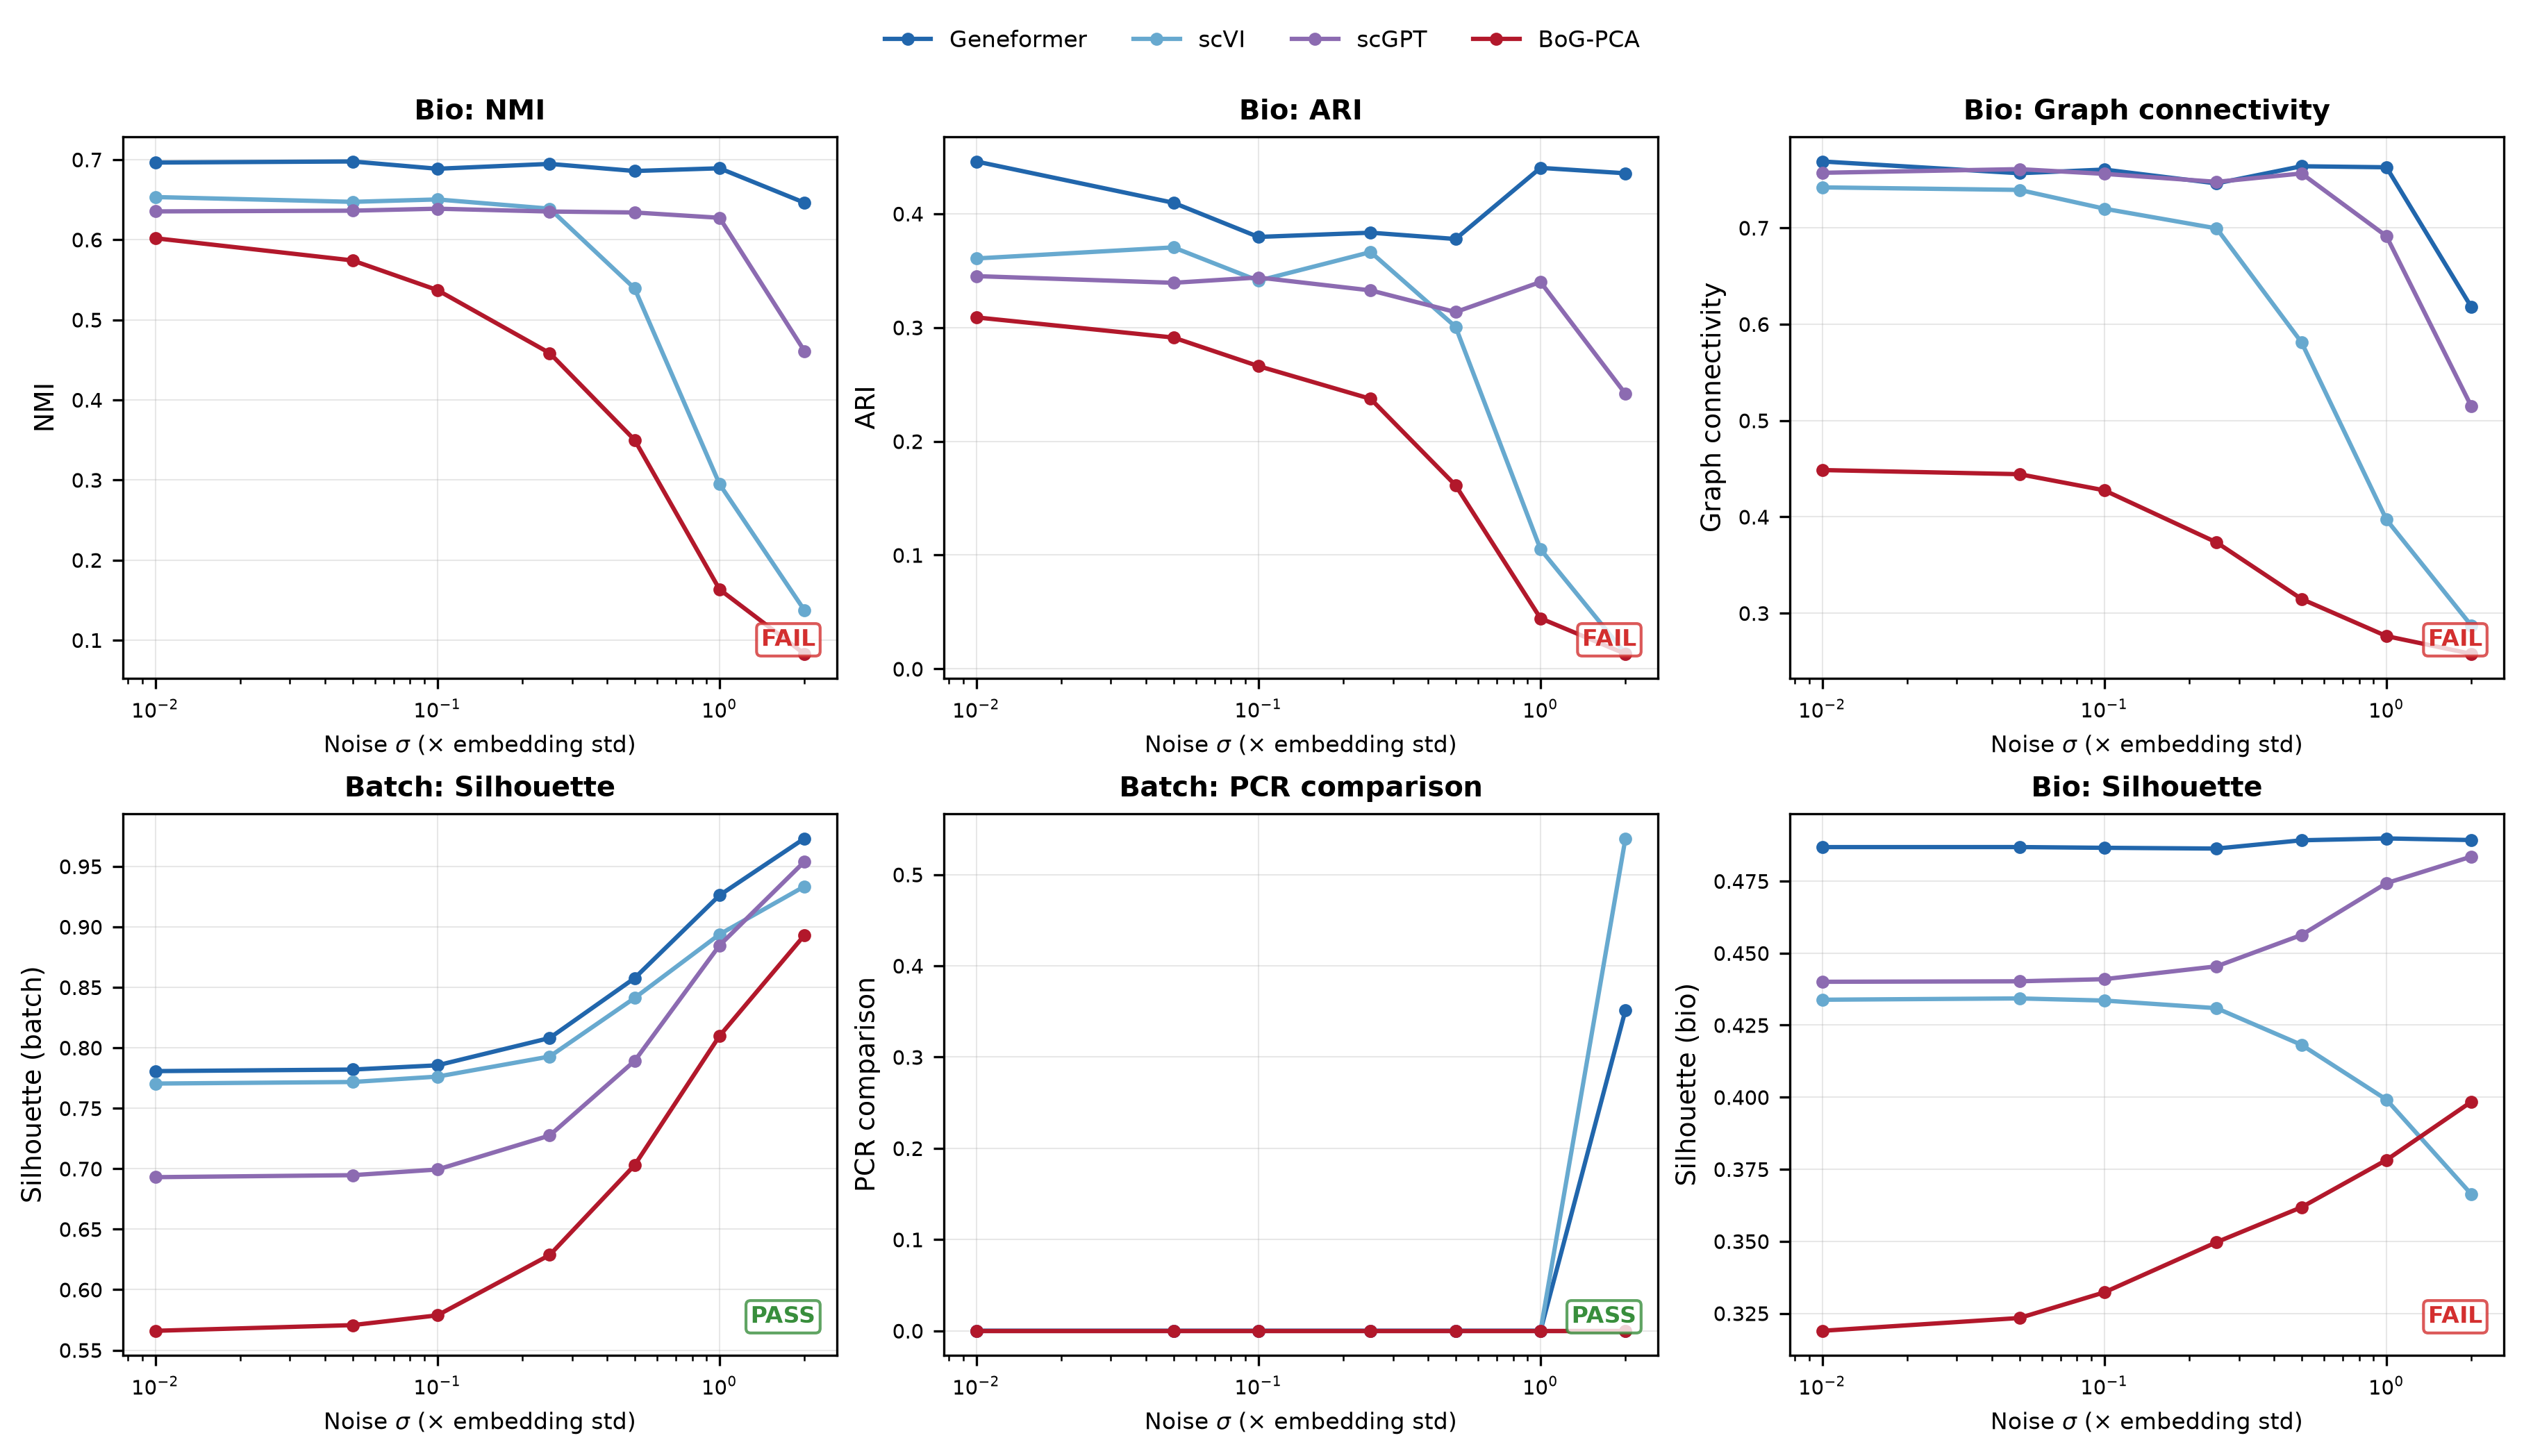
\includegraphics[width=\textwidth]{figures/noise_dose_response.pdf}
\caption{Noise dose-response curves for six scIB metrics on lung
embeddings (4 trained models). Bio-conservation metrics (top row)
show non-monotonic behavior: scores increase at intermediate noise
levels before declining, indicating sensitivity to clustering
artifacts. Batch-correction metrics (bottom center, right) decrease
monotonically as expected. Each curve traces a single embedding model
across seven noise magnitudes ($\sigma$ in units of embedding standard
deviation).}
\label{fig:noise_dose}
\end{figure}

\medskip
\begin{table}[h!]
\centering
\caption{Noise dose-response: raw vs.\ null-calibrated
non-monotonicity across 120 conditions (22 tissues $\times$ $\sim$6
embeddings, 10 seeds). Raw: fraction with mean $H > 0.01$ (metric
increased at some noise level). Calibrated: fraction exceeding the
permutation null ($\alpha = 0.01$, 1{,}000 $\sigma$-label
permutations). The inflation ratio quantifies how much uncalibrated
analysis overstates genuine non-monotonicity.}
\label{tab:noise}
\small
\begin{tabular}{@{}lccc@{}}
\toprule
Metric & Raw positive & Calibrated & Inflation \\
\midrule
ARI (Leiden)         & 84/120 (70\%) &  8/120 (6.7\%)  & 10.5$\times$ \\
Graph connectivity   & 58/120 (48\%) &  3/120 (2.5\%)  & 19.3$\times$ \\
NMI (Leiden)         & 28/120 (23\%) &  4/120 (3.3\%)  &  7.0$\times$ \\
\midrule
Cell-type CKA        & 58/120 (48\%) & 34/120 (28\%)   &  1.7$\times$ \\
Procrustes           & 56/120 (47\%) & 37/120 (31\%)   &  1.5$\times$ \\
\midrule
Isolated label ASW   & 32/120 (27\%) & 31/120 (26\%)   &  1.0$\times$ \\
Silhouette (label)   & 52/120 (43\%) & 49/120 (41\%)   &  1.1$\times$ \\
\bottomrule
\end{tabular}
\end{table}

Multi-seed calibration shows that apparent non-monotonicity in
Leiden-dependent metrics is almost entirely clustering jitter. ARI
drops from 70\% raw non-monotonic to 6.7\% after calibration
(10.5$\times$ inflation); graph connectivity drops from 48\% to 2.5\%
(19.3$\times$). Noise drives cells into fewer Leiden clusters,
mechanically raising NMI, and smooths local neighborhoods, transiently
increasing graph connectivity. These per-seed increases are real but
do not exceed what random permutation of $\sigma$ labels produces.

Similarity metrics (CKA, Procrustes) and label-based metrics
(isolated-label ASW, silhouette) show modest inflation
(1.0--1.7$\times$), indicating that their non-monotonicity, where it
occurs, reflects a genuine response to noise.

\begin{figure}[h!]
\centering
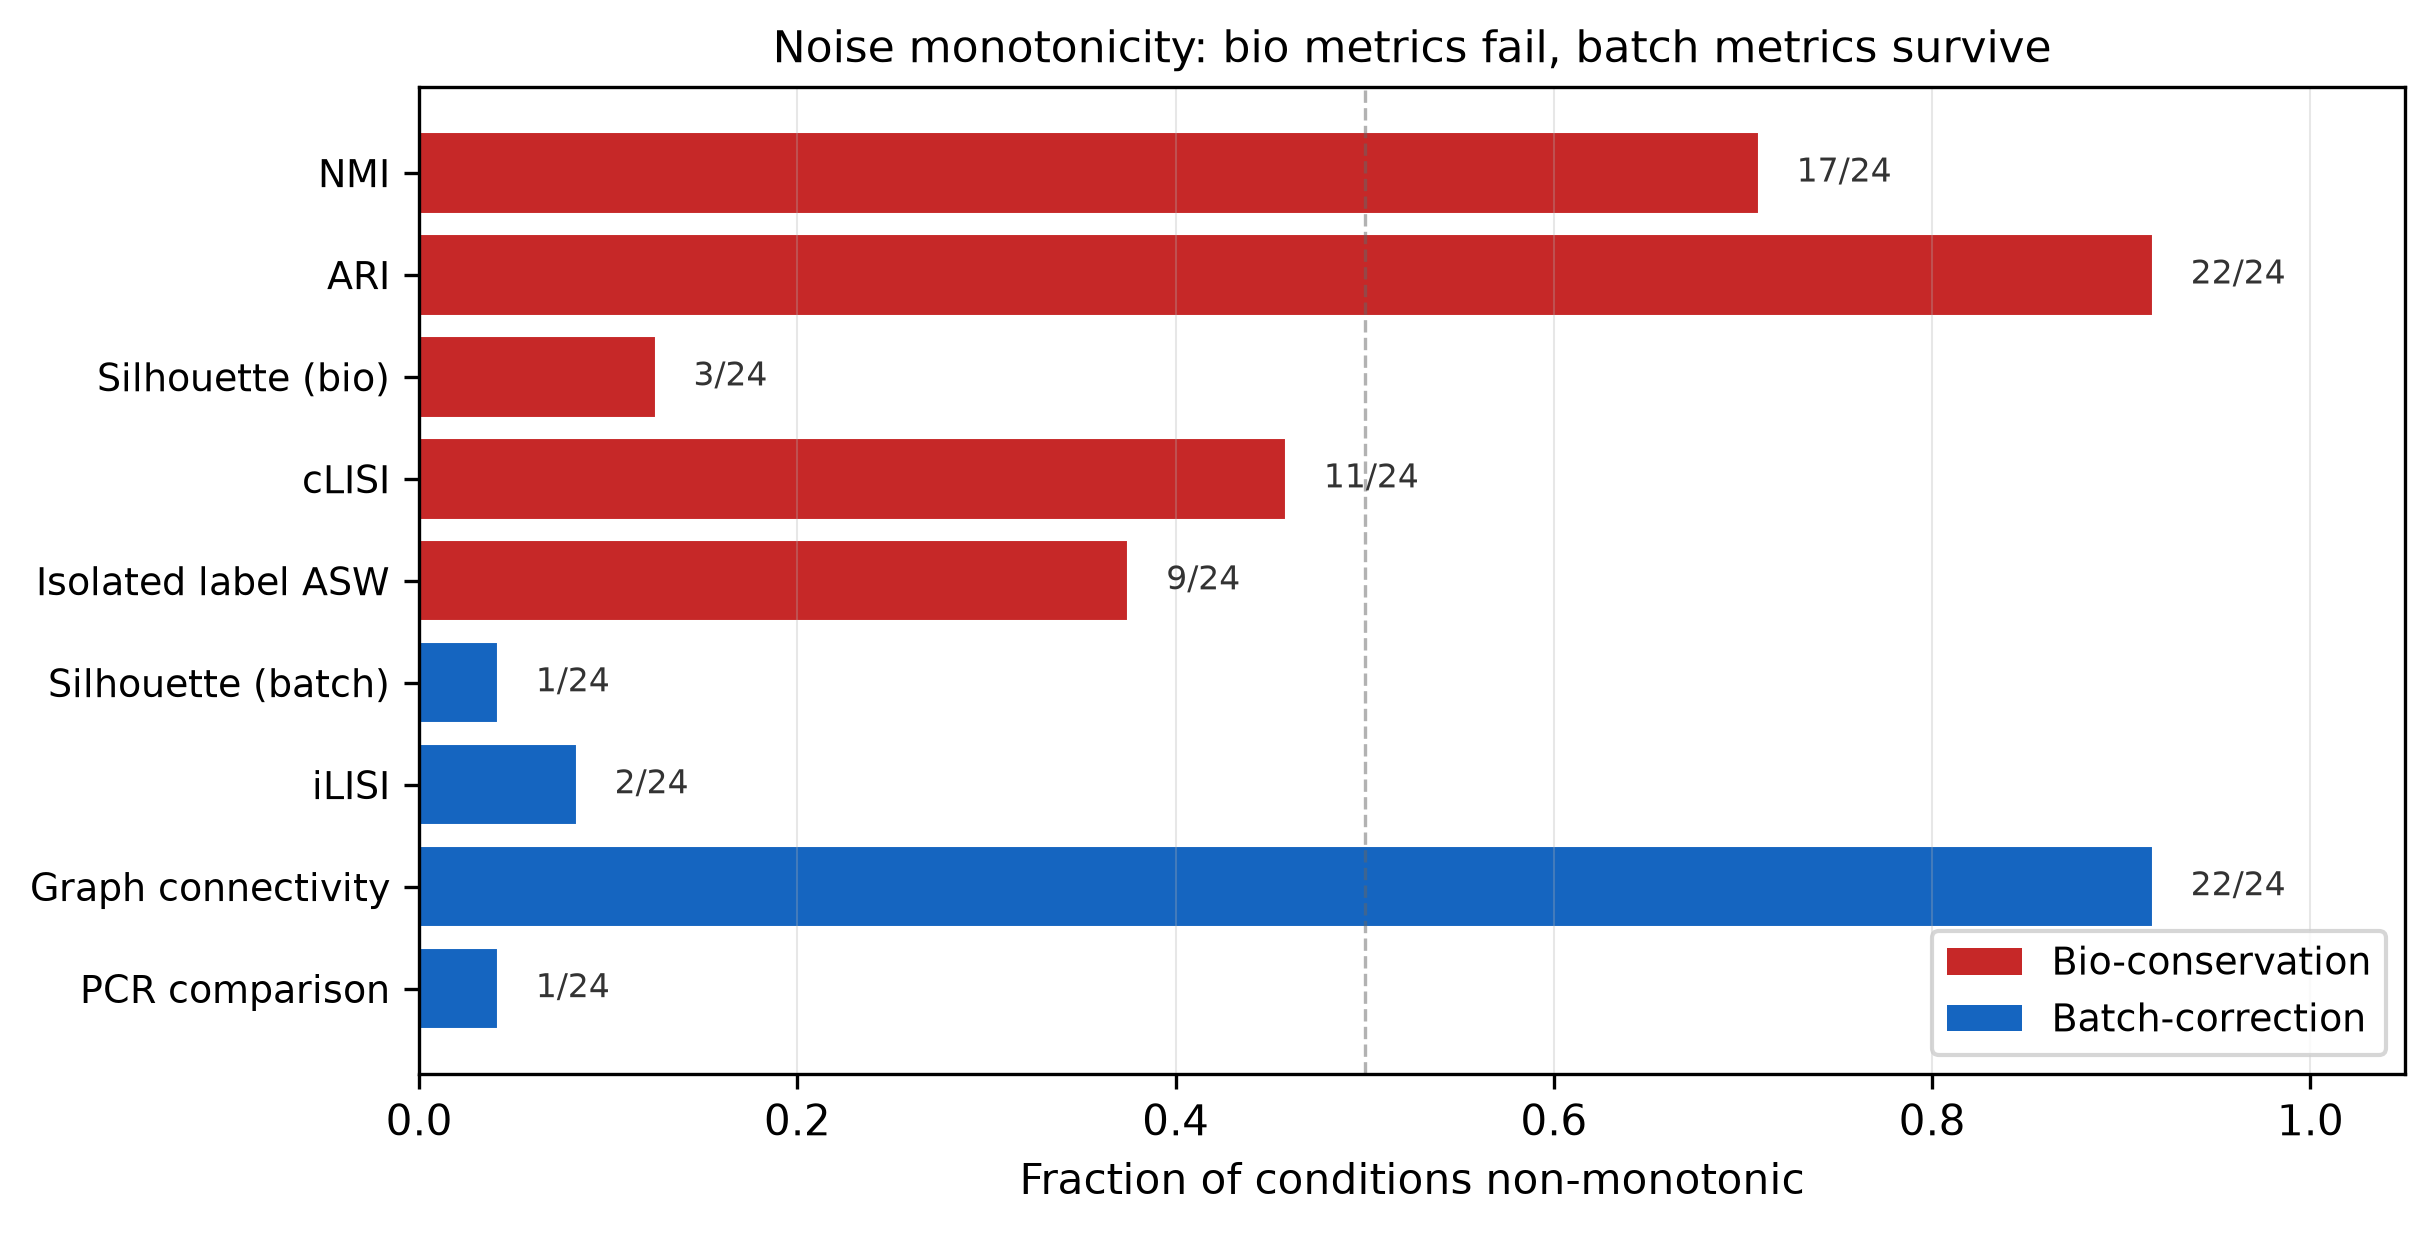
\includegraphics[width=0.85\textwidth]{figures/monotonicity_summary.pdf}
\caption{Fraction of embedding conditions (tissue $\times$ model)
exhibiting non-monotonic noise response, by metric. Bio-conservation
metrics (red) are non-monotonic in 25--75\% of conditions;
batch-correction metrics (blue) are non-monotonic in fewer than 15\%.
Counts are uncalibrated; Table~\ref{tab:noise} reports the calibrated
fractions after permutation testing.}
\label{fig:monotonicity}
\end{figure}

\paragraph{Single-seed trajectories.}
Table~\ref{tab:app_noise_fail} shows representative single-seed
non-monotonic trajectories illustrating the clustering jitter that
multi-seed calibration eliminates. NMI in brain/Geneformer shows scores
\emph{increasing} at high noise ($\sigma \geq 1.0$): noise drives all
cells into fewer Leiden clusters, mechanically raising NMI. These
per-seed trajectory changes are real but do not exceed what random
permutation of noise labels produces.

\medskip
\begin{table}[h!]
\centering
\caption{Representative single-seed non-monotonic trajectories. Values
are metric scores at $\sigma \in \{0.01, 0.05, 0.1, 0.25, 0.5, 1.0,
2.0\} \times \text{embedding\_std}$. Multi-seed calibration
(Table~\ref{tab:noise}) shows these patterns do not survive permutation
testing.}
\label{tab:app_noise_fail}
\footnotesize
\begin{tabular}{@{}llp{0.6\textwidth}@{}}
\toprule
Metric & Condition & $\sigma$: 0.01, 0.05, 0.1, 0.25, 0.5, 1.0, 2.0 \\
\midrule
Graph conn. & brain / scgpt & 0.772, 0.771, 0.773, \textbf{0.777}, \textbf{0.793}, 0.748, 0.589 \\
NMI & brain / geneformer & 0.550, 0.550, 0.545, \textbf{0.547}, 0.545, \textbf{0.575}, \textbf{0.577} \\
ARI & kidney / scvi & 0.397, \textbf{0.410}, 0.394, 0.351, 0.224, 0.073, 0.012 \\
cLISI & lung / scvi & 0.999, 0.999, \textbf{0.999}, 0.998, 0.975, 0.871, 0.642 \\
\bottomrule
\end{tabular}
\end{table}




\bibliographystyle{plainnat}
\bibliography{paper_d_v11}

\end{document}
